\documentclass[12pt]{article}
%Fall 2022
% Some basic packages
\usepackage{standalone}[subpreambles=true]
\usepackage[utf8]{inputenc}
\usepackage[T1]{fontenc}
\usepackage{textcomp}
\usepackage[english]{babel}
\usepackage{url}
\usepackage{graphicx}
%\usepackage{quiver}
\usepackage{float}
\usepackage{enumitem}
\usepackage{lmodern}
\usepackage{comment}
\usepackage{hyperref}
\usepackage[usenames,svgnames,dvipsnames]{xcolor}
\usepackage[margin=1in]{geometry}
\usepackage{pdfpages}

\pdfminorversion=7

% Don't indent paragraphs, leave some space between them
\usepackage{parskip}

% Hide page number when page is empty
\usepackage{emptypage}
\usepackage{subcaption}
\usepackage{multicol}
\usepackage[b]{esvect}

% Math stuff
\usepackage{amsmath, amsfonts, mathtools, amsthm, amssymb}
\usepackage{bbm}
\usepackage{stmaryrd}
\allowdisplaybreaks

% Fancy script capitals
\usepackage{mathrsfs}
\usepackage{cancel}
% Bold math
\usepackage{bm}
% Some shortcuts
\newcommand{\rr}{\ensuremath{\mathbb{R}}}
\newcommand{\zz}{\ensuremath{\mathbb{Z}}}
\newcommand{\qq}{\ensuremath{\mathbb{Q}}}
\newcommand{\nn}{\ensuremath{\mathbb{N}}}
\newcommand{\ff}{\ensuremath{\mathbb{F}}}
\newcommand{\cc}{\ensuremath{\mathbb{C}}}
\newcommand{\ee}{\ensuremath{\mathbb{E}}}
\newcommand{\hh}{\ensuremath{\mathbb{H}}}
\renewcommand\O{\ensuremath{\emptyset}}
\newcommand{\norm}[1]{{\left\lVert{#1}\right\rVert}}
\newcommand{\dbracket}[1]{{\left\llbracket{#1}\right\rrbracket}}
\newcommand{\ve}[1]{{\bm{#1}}}
\newcommand\allbold[1]{{\boldmath\textbf{#1}}}
\DeclareMathOperator{\lcm}{lcm}
\DeclareMathOperator{\im}{im}
\DeclareMathOperator{\coim}{coim}
\DeclareMathOperator{\dom}{dom}
\DeclareMathOperator{\tr}{tr}
\DeclareMathOperator{\rank}{rank}
\DeclareMathOperator*{\var}{Var}
\DeclareMathOperator*{\ev}{E}
\DeclareMathOperator{\dg}{deg}
\DeclareMathOperator{\aff}{aff}
\DeclareMathOperator{\conv}{conv}
\DeclareMathOperator{\inte}{int}
\DeclareMathOperator*{\argmin}{argmin}
\DeclareMathOperator*{\argmax}{argmax}
\DeclareMathOperator{\graph}{graph}
\DeclareMathOperator{\sgn}{sgn}
\DeclareMathOperator*{\Rep}{Rep}
\DeclareMathOperator{\Proj}{Proj}
\DeclareMathOperator{\mat}{mat}
\DeclareMathOperator{\diag}{diag}
\DeclareMathOperator{\aut}{Aut}
\DeclareMathOperator{\gal}{Gal}
\DeclareMathOperator{\inn}{Inn}
\DeclareMathOperator{\edm}{End}
\DeclareMathOperator{\Hom}{Hom}
\DeclareMathOperator{\ext}{Ext}
\DeclareMathOperator{\tor}{Tor}
\DeclareMathOperator{\Span}{Span}
\DeclareMathOperator{\Stab}{Stab}
\DeclareMathOperator{\cont}{cont}
\DeclareMathOperator{\Ann}{Ann}
\DeclareMathOperator{\Div}{div}
\DeclareMathOperator{\curl}{curl}
\DeclareMathOperator{\nat}{Nat}
\DeclareMathOperator{\gr}{Gr}
\DeclareMathOperator{\vect}{Vect}
\DeclareMathOperator{\id}{id}
\DeclareMathOperator{\Mod}{Mod}
\DeclareMathOperator{\sign}{sign}
\DeclareMathOperator{\Surf}{Surf}
\DeclareMathOperator{\fcone}{fcone}
\DeclareMathOperator{\Rot}{Rot}
\DeclareMathOperator{\grad}{grad}
\DeclareMathOperator{\atan2}{atan2}
\DeclareMathOperator{\Ric}{Ric}
\let\vec\relax
\DeclareMathOperator{\vec}{vec}
\let\Re\relax
\DeclareMathOperator{\Re}{Re}
\let\Im\relax
\DeclareMathOperator{\Im}{Im}
% Put x \to \infty below \lim
\let\svlim\lim\def\lim{\svlim\limits}

%wide hat
\usepackage{scalerel,stackengine}
\stackMath
\newcommand*\wh[1]{%
\savestack{\tmpbox}{\stretchto{%
  \scaleto{%
    \scalerel*[\widthof{\ensuremath{#1}}]{\kern-.6pt\bigwedge\kern-.6pt}%
    {\rule[-\textheight/2]{1ex}{\textheight}}%WIDTH-LIMITED BIG WEDGE
  }{\textheight}% 
}{0.5ex}}%
\stackon[1pt]{#1}{\tmpbox}%
}
\parskip 1ex

%Make implies and impliedby shorter
\let\implies\Rightarrow
\let\impliedby\Leftarrow
\let\iff\Leftrightarrow
\let\epsilon\varepsilon

% Add \contra symbol to denote contradiction
\usepackage{stmaryrd} % for \lightning
\newcommand\contra{\scalebox{1.5}{$\lightning$}}

% \let\phi\varphi

% Command for short corrections
% Usage: 1+1=\correct{3}{2}

\definecolor{correct}{HTML}{009900}
\newcommand\correct[2]{\ensuremath{\:}{\color{red}{#1}}\ensuremath{\to }{\color{correct}{#2}}\ensuremath{\:}}
\newcommand\green[1]{{\color{correct}{#1}}}

% horizontal rule
\newcommand\hr{
    \noindent\rule[0.5ex]{\linewidth}{0.5pt}
}

% hide parts
\newcommand\hide[1]{}

% si unitx
\usepackage{siunitx}
\sisetup{locale = FR}

%allows pmatrix to stretch
\makeatletter
\renewcommand*\env@matrix[1][\arraystretch]{%
  \edef\arraystretch{#1}%
  \hskip -\arraycolsep
  \let\@ifnextchar\new@ifnextchar
  \array{*\c@MaxMatrixCols c}}
\makeatother

\renewcommand{\arraystretch}{0.8}

\renewcommand{\baselinestretch}{1.5}

\usepackage{graphics}
\usepackage{epstopdf}

\RequirePackage{hyperref}
%%
%% Add support for color in order to color the hyperlinks.
%% 
\hypersetup{
  colorlinks = true,
  urlcolor = blue,
  citecolor = blue
}
%%fakesection Links
\hypersetup{
    colorlinks,
    linkcolor={red!50!black},
    citecolor={green!50!black},
    urlcolor={blue!80!black}
}
%customization of cleveref
\RequirePackage[capitalize,nameinlink]{cleveref}[0.19]

% Per SIAM Style Manual, "section" should be lowercase
\crefname{section}{section}{sections}
\crefname{subsection}{subsection}{subsections}
\Crefname{section}{Section}{Sections}
\Crefname{subsection}{Subsection}{Subsections}

% Per SIAM Style Manual, "Figure" should be spelled out in references
\Crefname{figure}{Figure}{Figures}

% Per SIAM Style Manual, don't say equation in front on an equation.
\crefformat{equation}{\textup{#2(#1)#3}}
\crefrangeformat{equation}{\textup{#3(#1)#4--#5(#2)#6}}
\crefmultiformat{equation}{\textup{#2(#1)#3}}{ and \textup{#2(#1)#3}}
{, \textup{#2(#1)#3}}{, and \textup{#2(#1)#3}}
\crefrangemultiformat{equation}{\textup{#3(#1)#4--#5(#2)#6}}%
{ and \textup{#3(#1)#4--#5(#2)#6}}{, \textup{#3(#1)#4--#5(#2)#6}}{, and \textup{#3(#1)#4--#5(#2)#6}}

% But spell it out at the beginning of a sentence.
\Crefformat{equation}{#2Equation~\textup{(#1)}#3}
\Crefrangeformat{equation}{Equations~\textup{#3(#1)#4--#5(#2)#6}}
\Crefmultiformat{equation}{Equations~\textup{#2(#1)#3}}{ and \textup{#2(#1)#3}}
{, \textup{#2(#1)#3}}{, and \textup{#2(#1)#3}}
\Crefrangemultiformat{equation}{Equations~\textup{#3(#1)#4--#5(#2)#6}}%
{ and \textup{#3(#1)#4--#5(#2)#6}}{, \textup{#3(#1)#4--#5(#2)#6}}{, and \textup{#3(#1)#4--#5(#2)#6}}

% Make number non-italic in any environment.
\crefdefaultlabelformat{#2\textup{#1}#3}

% Environments
\makeatother
% For box around Definition, Theorem, \ldots
%%fakesection Theorems
\usepackage{thmtools}
\usepackage[framemethod=TikZ]{mdframed}

\theoremstyle{definition}
\mdfdefinestyle{mdbluebox}{%
	roundcorner = 10pt,
	linewidth=1pt,
	skipabove=12pt,
	innerbottommargin=9pt,
	skipbelow=2pt,
	nobreak=true,
	linecolor=blue,
	backgroundcolor=TealBlue!5,
}
\declaretheoremstyle[
	headfont=\sffamily\bfseries\color{MidnightBlue},
	mdframed={style=mdbluebox},
	headpunct={\\[3pt]},
	postheadspace={0pt}
]{thmbluebox}

\mdfdefinestyle{mdredbox}{%
	linewidth=0.5pt,
	skipabove=12pt,
	frametitleaboveskip=5pt,
	frametitlebelowskip=0pt,
	skipbelow=2pt,
	frametitlefont=\bfseries,
	innertopmargin=4pt,
	innerbottommargin=8pt,
	nobreak=false,
	linecolor=RawSienna,
	backgroundcolor=Salmon!5,
}
\declaretheoremstyle[
	headfont=\bfseries\color{RawSienna},
	mdframed={style=mdredbox},
	headpunct={\\[3pt]},
	postheadspace={0pt},
]{thmredbox}

\declaretheorem[%
style=thmbluebox,name=Theorem,numberwithin=section]{thm}
\declaretheorem[style=thmbluebox,name=Lemma,sibling=thm]{lem}
\declaretheorem[style=thmbluebox,name=Proposition,sibling=thm]{prop}
\declaretheorem[style=thmbluebox,name=Corollary,sibling=thm]{coro}
\declaretheorem[style=thmredbox,name=Example,sibling=thm]{eg}

\mdfdefinestyle{mdgreenbox}{%
	roundcorner = 10pt,
	linewidth=1pt,
	skipabove=12pt,
	innerbottommargin=9pt,
	skipbelow=2pt,
	nobreak=true,
	linecolor=ForestGreen,
	backgroundcolor=ForestGreen!5,
}

\declaretheoremstyle[
	headfont=\bfseries\sffamily\color{ForestGreen!70!black},
	bodyfont=\normalfont,
	spaceabove=2pt,
	spacebelow=1pt,
	mdframed={style=mdgreenbox},
	headpunct={ --- },
]{thmgreenbox}

\declaretheorem[style=thmgreenbox,name=Definition,sibling=thm]{defn}

\mdfdefinestyle{mdgreenboxsq}{%
	linewidth=1pt,
	skipabove=12pt,
	innerbottommargin=9pt,
	skipbelow=2pt,
	nobreak=true,
	linecolor=ForestGreen,
	backgroundcolor=ForestGreen!5,
}
\declaretheoremstyle[
	headfont=\bfseries\sffamily\color{ForestGreen!70!black},
	bodyfont=\normalfont,
	spaceabove=2pt,
	spacebelow=1pt,
	mdframed={style=mdgreenboxsq},
	headpunct={},
]{thmgreenboxsq}
\declaretheoremstyle[
	headfont=\bfseries\sffamily\color{ForestGreen!70!black},
	bodyfont=\normalfont,
	spaceabove=2pt,
	spacebelow=1pt,
	mdframed={style=mdgreenboxsq},
	headpunct={},
]{thmgreenboxsq*}

\mdfdefinestyle{mdblackbox}{%
	skipabove=8pt,
	linewidth=3pt,
	rightline=false,
	leftline=true,
	topline=false,
	bottomline=false,
	linecolor=black,
	backgroundcolor=RedViolet!5!gray!5,
}
\declaretheoremstyle[
	headfont=\bfseries,
	bodyfont=\normalfont\small,
	spaceabove=0pt,
	spacebelow=0pt,
	mdframed={style=mdblackbox}
]{thmblackbox}

\theoremstyle{plain}
\declaretheorem[name=Question,sibling=thm,style=thmblackbox]{ques}
\declaretheorem[name=Remark,sibling=thm,style=thmgreenboxsq]{remark}
\declaretheorem[name=Remark,sibling=thm,style=thmgreenboxsq*]{remark*}
\newtheorem{ass}[thm]{Assumptions}

\theoremstyle{definition}
\newtheorem*{problem}{Problem}
\newtheorem{claim}[thm]{Claim}
\theoremstyle{remark}
\newtheorem*{case}{Case}
\newtheorem*{notation}{Notation}
\newtheorem*{note}{Note}
\newtheorem*{motivation}{Motivation}
\newtheorem*{intuition}{Intuition}
\newtheorem*{conjecture}{Conjecture}

% Make section starts with 1 for report type
%\renewcommand\thesection{\arabic{section}}

% End example and intermezzo environments with a small diamond (just like proof
% environments end with a small square)
\usepackage{etoolbox}
\AtEndEnvironment{vb}{\null\hfill$\diamond$}%
\AtEndEnvironment{intermezzo}{\null\hfill$\diamond$}%
% \AtEndEnvironment{opmerking}{\null\hfill$\diamond$}%

% Fix some spacing
% http://tex.stackexchange.com/questions/22119/how-can-i-change-the-spacing-before-theorems-with-amsthm
\makeatletter
\def\thm@space@setup{%
  \thm@preskip=\parskip \thm@postskip=0pt
}

% Fix some stuff
% %http://tex.stackexchange.com/questions/76273/multiple-pdfs-with-page-group-included-in-a-single-page-warning
\pdfsuppresswarningpagegroup=1


% My name
\author{Jaden Wang}


%include Matlab code
\usepackage{sectsty}
\usepackage{listings}
\usepackage{color}
\usepackage{alltt}
\definecolor{dkgreen}{rgb}{0,0.6,0}
\definecolor{gray}{rgb}{0.5,0.5,0.5}
\definecolor{mauve}{rgb}{0.58,0,0.82}

\lstset{frame=tb,
  language=Matlab,
  aboveskip=3mm,
  belowskip=3mm,
  showstringspaces=false,
  columns=flexible,
  basicstyle={\small\ttfamily},
  numbers=none,
  numberstyle=\tiny\color{gray},
  keywordstyle=\color{blue},
  commentstyle=\color{dkgreen},
  stringstyle=\color{mauve},
  breaklines=true,
  breakatwhitespace=true,
  tabsize=3
}
\begin{document}
\centerline {\textsf{\textbf{\LARGE{Homework 6}}}}
\centerline {Jaden Wang}
\vspace{.15in}
\begin{problem}[1]
From the example, we know that optimal trajectories are clockwise-oriented circles centered at $ ( 1,0)$ for $ u=1$  and centered at $ (-1,0)$ for $ u = - 1$. To reach the origin, we must eventually get on the switching curves $ \Gamma_+^{1} $ and $ \Gamma_{-}^{1}$ since they are the only circles centered at $ (\pm1,0)$ that go through the origin. Moreover, the optimal control $ u^*  = - \text{sign}(\Lambda \cos(\omega t + \phi))$ flips signs and thus must switch every  $ \frac{\pi}{ \omega} = \pi$ except that it might switch sooner at the beginning or in the end. 

\begin{enumerate}[label=(\alph*)]
\item When $ x_1(0) = x_2(0)=2$, we have the following optimal trajectory:
~\begin{figure}[H]
	\centering
	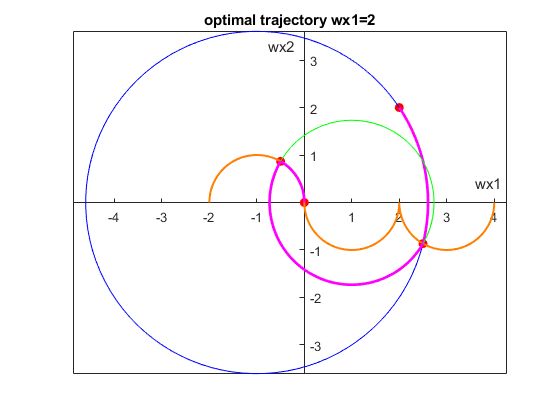
\includegraphics[width=0.6\textwidth]{./figures/6.1.png}
\caption{Magenta denotes the optimal trajectory and orange denotes the optimal switching curve. We first find clockwise-oriented circles centered at $ (\pm 1,0)$ that go through $ (2,2)$ and pick the one that reaches the switching surface the fastest. In this case it is the blue circle centered at  $ (-1,0)$. Then we switch to the green circle centered at $ (1,0)$ and continue for $ \pi$ unit of time to reach the next switching curve which happens to be $ \Gamma_{-}^{1}$ so we simply follow the singular curve to reach the origin.}
\end{figure}

Using $ \wh{ \Gamma}$, we have the following trajectory:
~\begin{figure}[H]
	\centering
	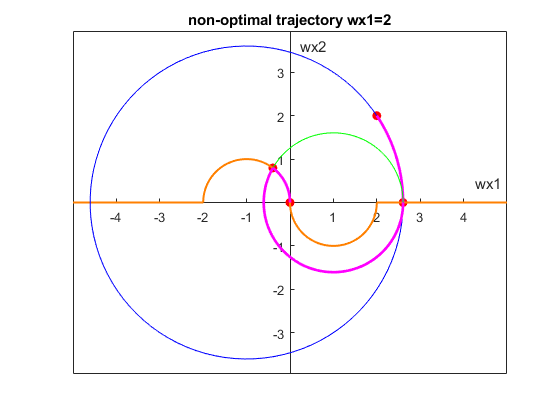
\includegraphics[width=0.6\textwidth]{./figures/6.2.png}
	\caption{Magenta denotes the non-optimal trajectory and orange denotes the non-optimal switching curve. We repeat the previous first step, reach a new switching curve at $ x_2=0$, and switch to the other center. This time we don't have to switch every $ \pi$ so we simply reach the next switching curve to switch.}
\end{figure}
Since $ \omega=1$, the elapsed time is the same as the angle the trajectory traced out. By adding the angles together, we obtain that $ t^*  = 5.0194$ and $ \wh{ t} = 5.1685$.
\item We repeat the procedure for $ \omega x_1 = 3,4,5$.
~\begin{figure}[H]
	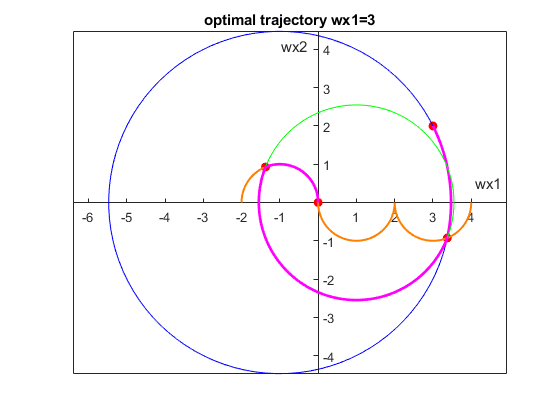
\includegraphics[width=0.49\textwidth]{./figures/6.3.png}
	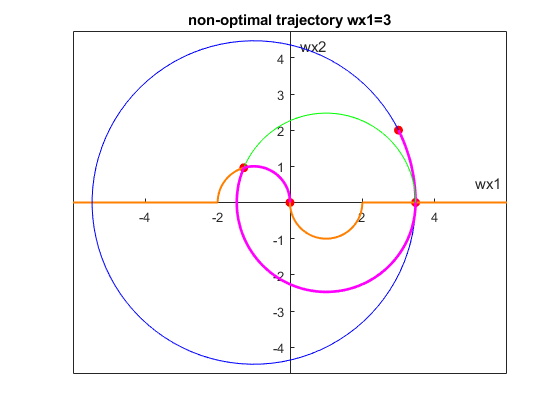
\includegraphics[width=0.49\textwidth]{./figures/6.4.png}
\end{figure}
~\begin{figure}[H]
	\centering
	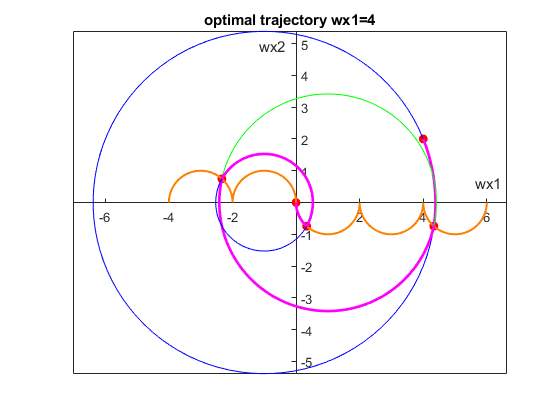
\includegraphics[width=0.49\textwidth]{./figures/6.5.png}
	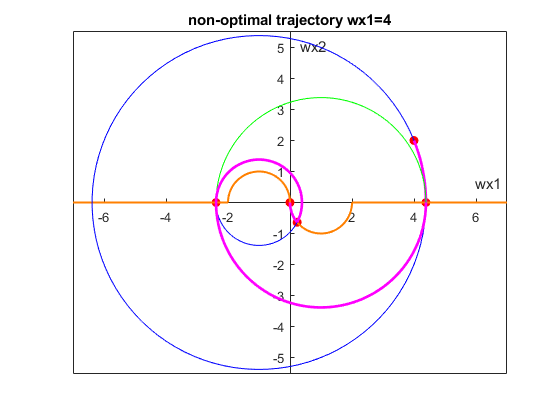
\includegraphics[width=0.49\textwidth]{./figures/6.6.png}
	\caption{Both trajectories becomes more complicated. We have four arcs corresponding to three switchings.}
\end{figure}
~\begin{figure}[H]
	\centering
	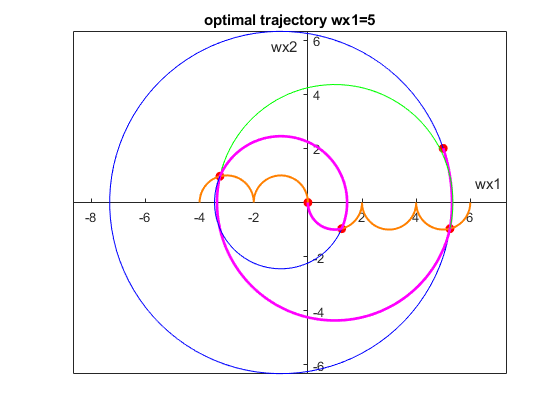
\includegraphics[width=0.49\textwidth]{./figures/6.7.png}
	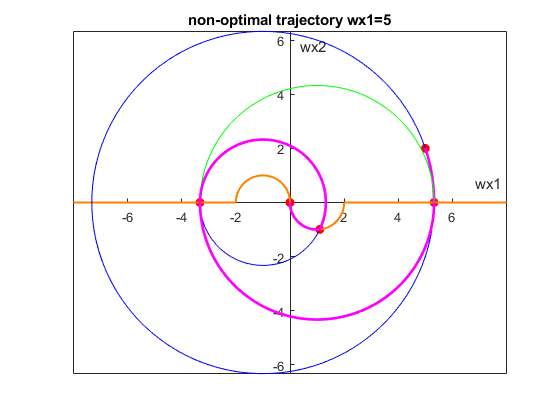
\includegraphics[width=0.49\textwidth]{./figures/6.8.png}
\end{figure}
From the figures, we can roughly see that the optimal trajectories and their non-optimal counterparts largely resembles each other. Moreover, it is not hard to imagine that as $ \omega x_1$ gets larger, the total angles traced out by both trajectories increase but their differences don't increase much. Thus the ratio $ \wh{ t} / t^* $ trends down to 1. There is not enough sample size in the following plot to fully illustrate that but it is a start:
~\begin{figure}[H]
	\centering
	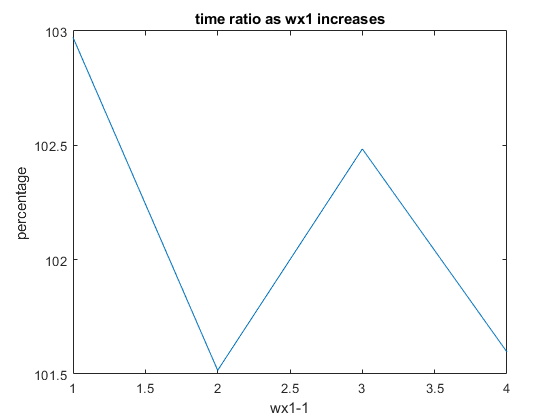
\includegraphics[width=0.55\textwidth]{./figures/6.15.png}
	\caption{The ratio fluctuates but trends down.}
\end{figure}

\end{enumerate}
\end{problem}


\begin{problem}[2]
The Hamiltonian is
\begin{align*}
	H &= \frac{1}{2} x_1^2 + p_1(x_2+u) + p_2(-u)\\
	&= \frac{1}{2}x_1^2+p_1x_2 +(p_1-p_2)u 
\end{align*}
The adjoint equations are
\begin{align*}
	\dot{p_1} &= -H_{x_1} = -x_1 \\
	\dot{p_2} &= -H_{x_2} = -p_1
\end{align*}
Since $ t_f$ is free, and  $ H$ is time-independent, transversality yields  $ H \equiv 0$. 

\begin{enumerate}[label=(\alph*)]
\item Let us examine the optimality condition. By the PMP,
\begin{align*}
	u^*  = \argmin_u H = \begin{cases}
		-1 & p_1 - p_2 >0\\
		? & p_1 - p_2 =0\\
		1 & p_1 - p_2 <0
	\end{cases}
\end{align*}
Notice on the singular surface we have
\begin{align*}
	H = \frac{1}{2} x_1^2+x_1 x_2 &= 0 \\
	x_1(x_1+x_2) &= 0\\
	\implies x_1 =0 \text{ or } & x_1 = -2 x_2 
\end{align*}
Denote the surfaces by $ S_1$ and $ S_2$ respectively. Now we use GLC to obtain the optimal control on the singular surface
\begin{align*}
	\dot{H}_u &= \dot{p_1} - \dot{p_2} = -x_1 + p_1 \implies x_1 = p_1 = p_2 \\
	\ddot{H}_u &= -\dot{x_1} + \dot{p_1} = -x_2 - u - x_1 =0 \\
	u^* &= -(x_1 + x_2) 
\end{align*}
Moreover, since $ k=1$, $ (-1)^{1 } \frac{\partial }{\partial u} \ddot{H}_u = 1 >0 $ which passes GLC. Thus by definition of $ S_1$ and $S_2$,
\begin{align*}
	u^* = \begin{cases}
		-x_2 & \text{ on } S_1\\
		x_2 & \text{ on } S_2
	\end{cases}
\end{align*}
Notice that on $ S_1$, $ \dot{x_2} = x_2$ so $ x_2$ moves away from origin. On $ S_2$, we have
\begin{align*}
	\begin{cases}
		\dot{x_1} = 2x_2 \\
		\dot{x_2} = -x_2 \\
	\end{cases}
\end{align*}
which indicates that trajectory on $ S_2$ move toward the origin as time increases.
~\begin{figure}[H]
	\centering
	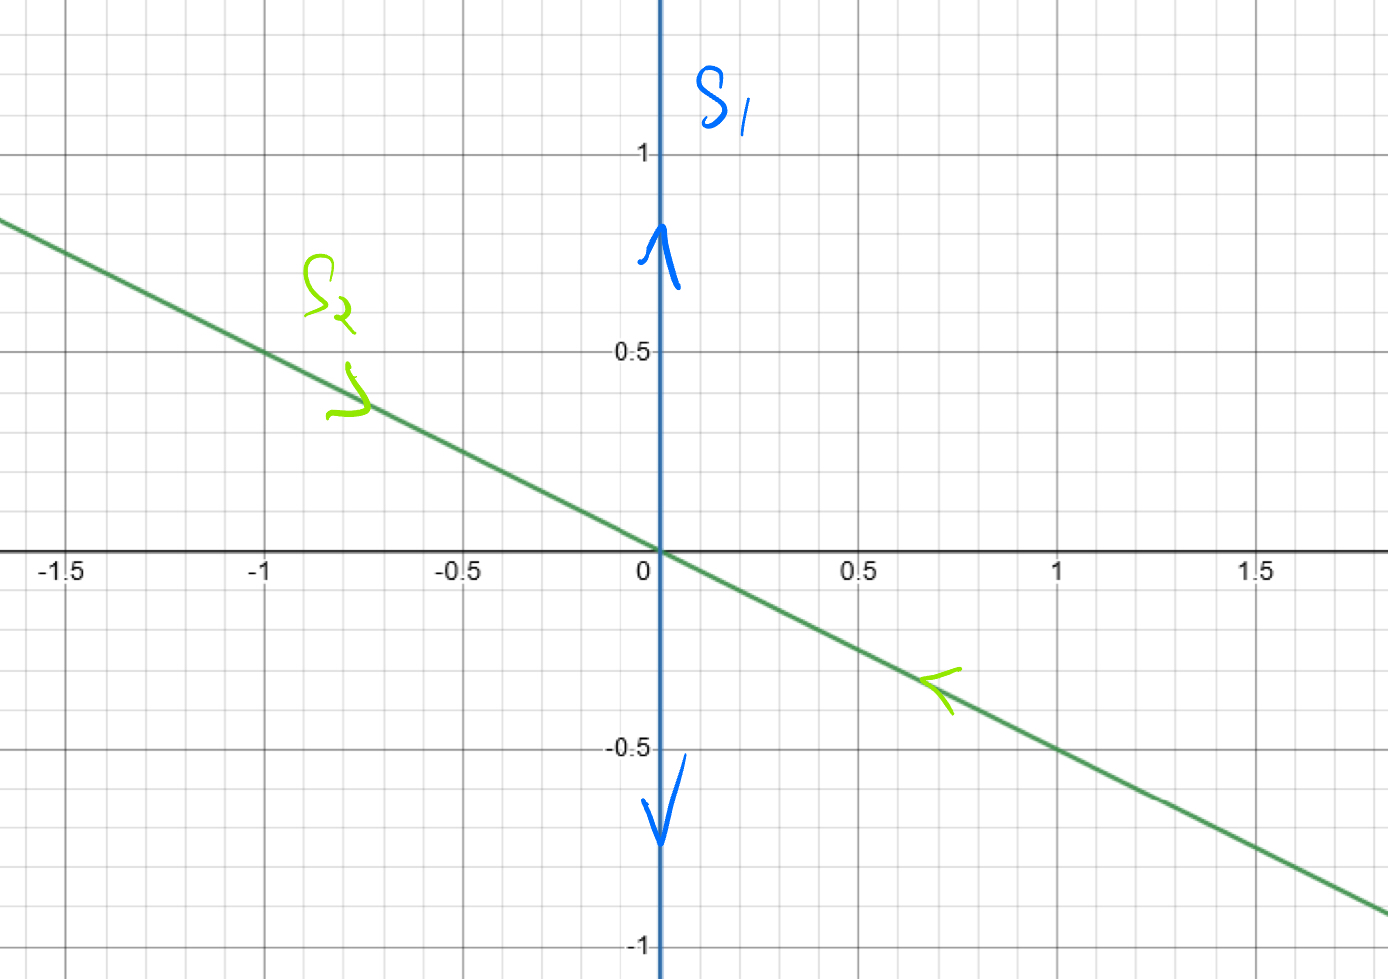
\includegraphics[width=0.6\textwidth]{./figures/6.16.png}
	\caption{Switching surfaces: $ S_1$ is blue and $ S_2$ is green.}
\end{figure}
Now the initial point $ (0,-0.5)$ is on $ S_1$, we cannot continue on $ S_1$ as it moves away from the target. Hence we resort to bang-bang control. If $ u=1$, dynamics are
\begin{align*}
	\begin{cases}
		\dot{x_1} = x_2 + 1 & x_1(0) = 0\\
		\dot{x_2} = -1 & x_2(0) = -\frac{1}{2}
	\end{cases}
\end{align*}
which yields $ x_1 = -\frac{1}{2} \left( x_2+\frac{1}{2} \right)^2 - \frac{1}{2}\left(x_2+\frac{1}{2}\right) $. However, both its intersections with $ x_1 = -2 x_2$ are not achieved in the positive time direction.

If $ u = -1$, the dynamics are
\begin{align*}	
	\begin{cases}
		\dot{x_1} = x_2 - 1 & x_1(0) = 0\\
		\dot{x_2} = 1 & x_2(0) = -\frac{1}{2}
	\end{cases}
\end{align*}
which yields
\begin{align*}
	\begin{cases}
		x_1 (t) = \frac{1}{2} t^2 - \frac{3}{2} t \\
		x_2(t) = t-\frac{1}{2} \implies t = x_2 + \frac{1}{2}
	\end{cases}
\end{align*}
so we have the trajectory $ x_1 = \frac{1}{2} \left( x+\frac{1}{2} \right)^2 - \frac{3}{2} \left( x_2 + \frac{1}{2} \right)  $. This intersections with $ S_2$ at $ (-1, 0.5)$ which is achieved in positive time $ t=1$. Thus at this time we switch to singular control.
~\begin{figure}[H]
	\centering
	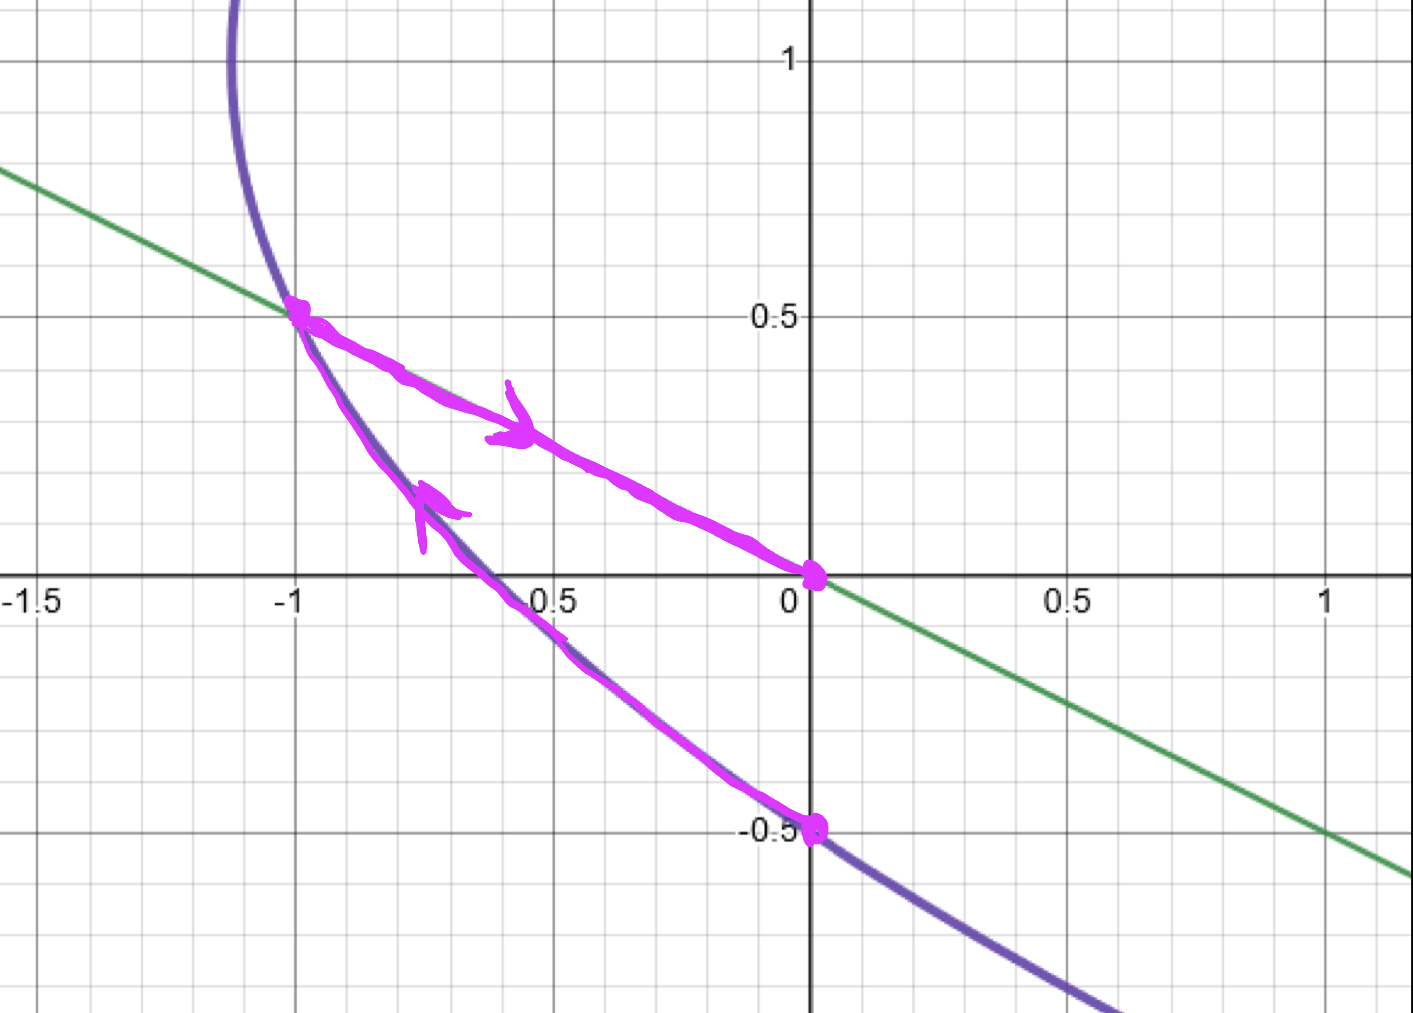
\includegraphics[width=0.6\textwidth]{./figures/6.17.png}
	\caption{Optimal trajectory from initial point $ (0, -0.5)$.}
\end{figure}
\item Yes we can use bang-bang control only to reach the origin. We simply use the bang-bang control $ u=-1$ above and then switch to $ u=1$ which it intersects a bang-bang trajectory using $ u=1$ that reaches the origin. We find the latter trajectory with reversed time so that it goes through the origin at $ t=0$ for simplicity:
\begin{align*}
	\begin{cases}
		\dot{x_1} = x_2 + 1 & x_1(0) = 0\\
		\dot{x_2} = -1 & x_2(0) = 0
	\end{cases}
\end{align*}
which yields
\begin{align*}
	\begin{cases}
		x_1 (t) =- \frac{1}{2} t^2 + t \\
		x_2(t) = -t \implies t = -x_2 
	\end{cases}
\end{align*}
This gives the trajectory $ x_1 = -\frac{1}{2} x_2^2 - x_2$. The two bang-bang arcs intersect at $ (-1.1031,0.7906)$, with  $ t = -0.7906$. Thus the trajectory is
~\begin{figure}[H]
	\centering
	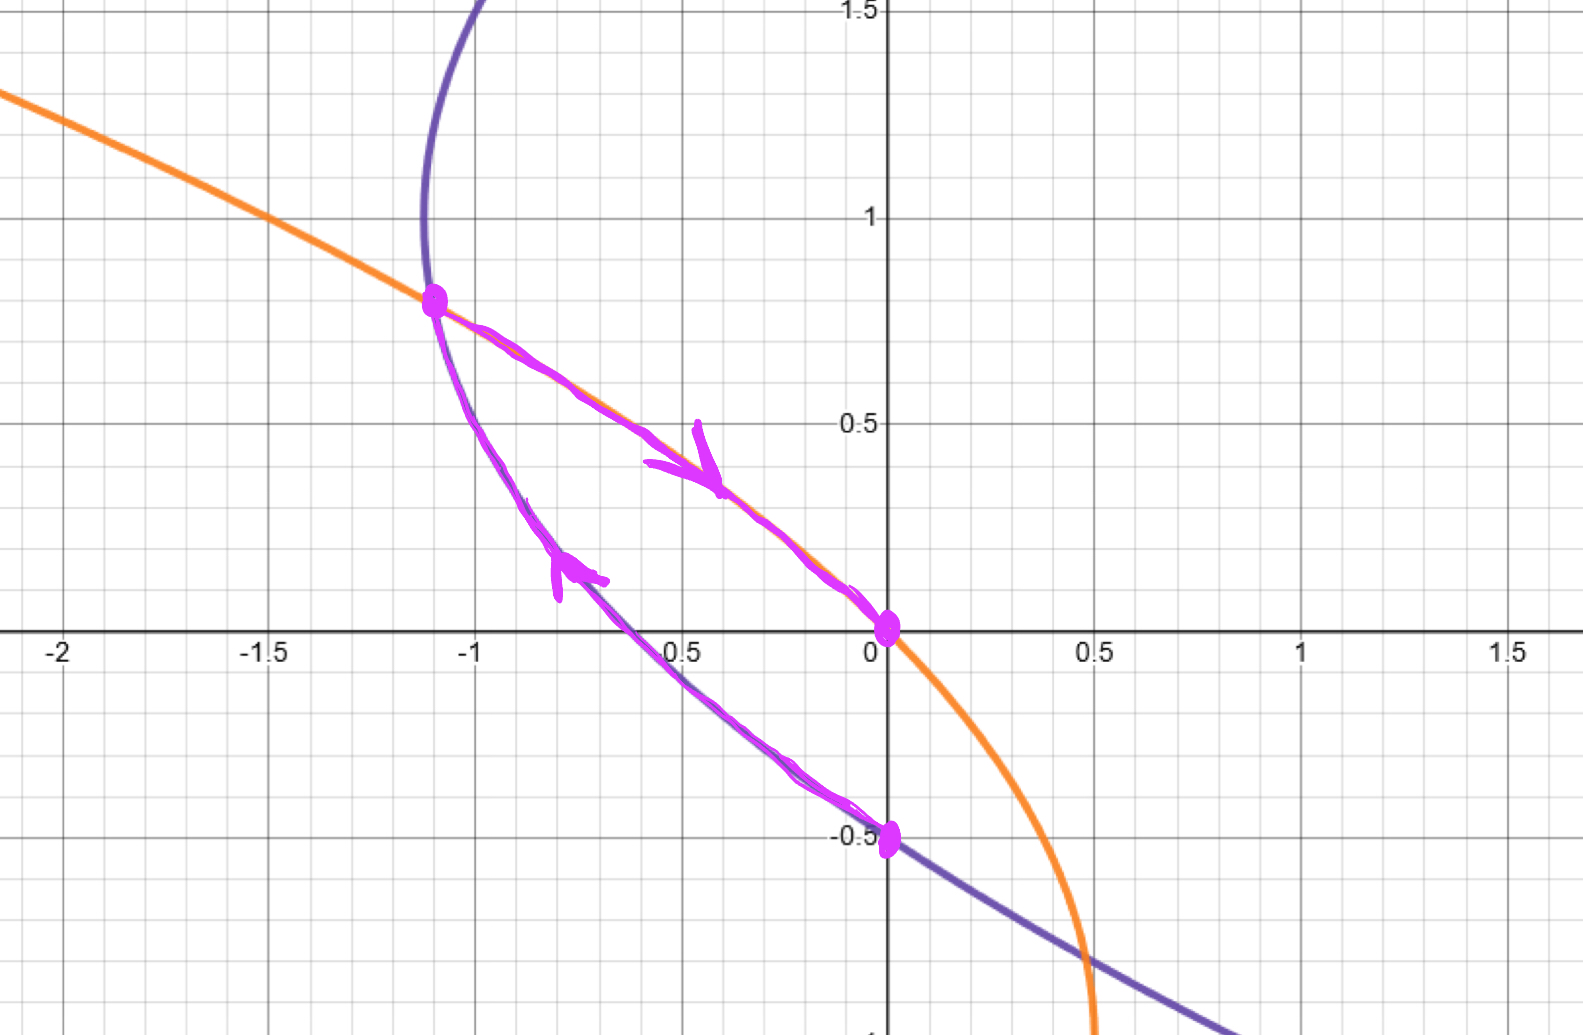
\includegraphics[width=0.6\textwidth]{./figures/6.18.png}
	\caption{Bang-bang only trajectory.}
	\label{fig:6-18-png}
\end{figure}
\item For the optimal control, we see that the first intersection occurs at $ t_1 = x_2 + \frac{1}{2} = 1$. Moreover, since $ x_1 = p_1$, the adjoint equation becomes $ x_1 = - \dot{x_1}$. Thus
\begin{align*}
	\frac{1}{2} \int_{ 1}^{ T} x_1^2 dt &= -\frac{1}{2} \int_{ 1}^{ T} x_1 \dot{x_1} dt \\
	&= -\frac{1}{2} \int_{ 1}^{ T} \frac{d}{dt} x_1 \dot{x_1} dt  \\
	&= -\frac{1}{4} \left( x_1(T)^2 - x_1(1)^2 \right)  \\
	&= \frac{1}{4} x_1(1)^2 \\
	&= \frac{1}{4} 
\end{align*}
and
\begin{align*}
	J^*  = \frac{1}{2} \int_{ 0}^{ T} x_1^2 dt &= \frac{1}{2} \int_{ 0}^{ 1} x_1^2 dt + \frac{1}{2} \int_{ 1}^{ T} x_1^2 dt \\
	&= \frac{1}{2} \int_{ 0}^{ 1} \left( \frac{1}{2} t^2 - \frac{3}{2}t \right)^2 dt + \frac{1}{4}   \\
	&= 0.4625 
\end{align*}

From (d) we obtain that for bang-bang trajectory, $ t_1= 1.2906$. Thus
\begin{align*}
	J_{BB} &= \frac{1}{2} \int_{ 0}^{ T} x_1^2 dt \\ 
	&= \frac{1}{2} \int_{ 0}^{ 1.2906} \left( \frac{1}{2} t^2 - \frac{3}{2}t \right)^2 dt + \frac{1}{2} \int_{ -0.7906}^{ 0} \left( \frac{1}{2} t^2 + t  \right)^2    \\
	&= 0.3755 + 0.1389 = 0.5144
\end{align*}
\item Solving the dynamics on $ S_2$ with boundary condition $ x_1(1) =-1, x_2(1)= \frac{1}{2}$ yields
\begin{align*}
	\begin{cases}
		x_1(t) = -2.7183 e^{-t}\\
		x_2(t) = 1.3591 e^{-t}
	\end{cases}
\end{align*}
which is never going to reach $ (0,0)$ in finite time.

In the bang-bang case, we have  $ t_1 = x_2 + \frac{1}{2} = 0.7906 + 0.5 = 1.2906$ so $ T = t_1 + 0.7906 = 2.0812$.
\end{enumerate}
\end{problem}

\begin{problem}[3]
The Hamiltonian is
\begin{align*}
	H = 1 + p_1 x_2 + p_2 u .
\end{align*}
The adjoint equations are
\begin{align*}
	\dot{p_1} &= -H_{x_1} = 0 \\
	\dot{p_2} &= -H_{x_2} = - p_1 
\end{align*}
We see that $ p_1$ is constant and $ p_2$ is linear.
\begin{enumerate}[label=(\alph*)]
\item By PMP, we know that the optimal control is
\begin{align*}
	u^*  = \argmin_u H = \begin{cases}
		u_{\max} & p_2 < 0\\
		? & p_2 =0\\
		-u_{\max} & p_2 >0
	\end{cases}
\end{align*}
Since $ p_2$ is linear, it cannot be zero for more than one point. Otherwise, $ p_2 = p_1 \equiv 0$ which implies that $ H \equiv 1$. However, since $ t_f$ is free, we have  $ H \equiv 0$, a contradiction. It follows that
 \begin{align*}
	u^* = - \text{sign}(p_2) \cdot u_{\max} = \pm u_{ \max},  
\end{align*}
\emph{i.e.} we only have bang-bang control.
\item Let $ b := \pm u_{\max}$. Thus the dynamics of optimal trajectory are
	\begin{align*}
		\begin{cases}
			\dot{x_2} = b &\implies x_2(t) = bt+x_{20}\\
			\dot{x_1} = x_2 &\implies x_1(t) = bt^2 + x_{20}t+x_{10}
		\end{cases}
	\end{align*}
By substitution we have the optimal trajectory
\begin{align*}
	x_1-\left( x_{10} -\frac{1}{2b} x_{20}^2\right)  = \frac{1}{2b} x_2^2 ,
\end{align*}
for initial point $ (x_{10},x_{20})$. To have end points at $ (0,\pm 1)$, the optimal trajectory must have its last arc on one of the orange parabolas below. These are the switching curves.
~\begin{figure}[H]
	\centering
	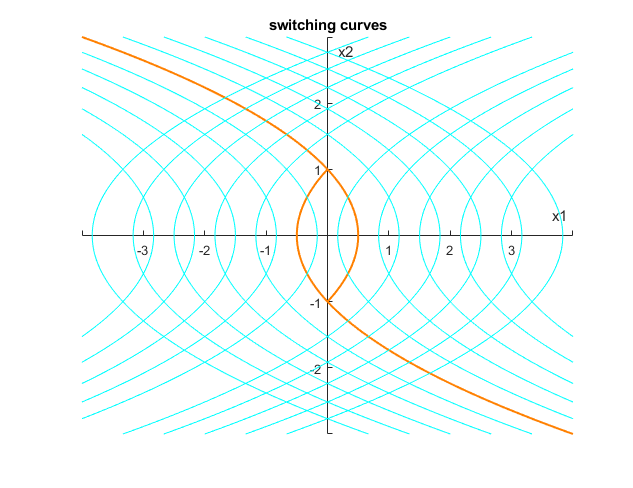
\includegraphics[width=0.7\textwidth]{./figures/6.9.png}
	\caption{The orange parabolas are the only optimal trajectories that go through $ (0,\pm 1)$. The cyan parabolas are other potential optimal trajectories. Given an initial point $ (x_{10},x_{20})$, there are always exactly two parabolas facing opposite directions that go through the point based on the equations above, and they always intersect at least one of the orange parabolas once. Note that the parabolas with mouth opening to the left goes down whereas the parabolas with mouth opening right goes up as time elapses. Note that the switching curves terminate after reaching $ (0,\pm 1)$. That is, the orange curve that goes up stops at  $ (0,1)$. The orange curve that goes down stops at $ (0,-1)$. This is because once they reach those points, they will never be able to return.}
\end{figure}
\item By the reasons stated in the caption above, yes solution exists for all initial points. They might not be unique, as the $ (0,0)$ case illustrates below.
\item 
~\begin{figure}[H]
	\centering
	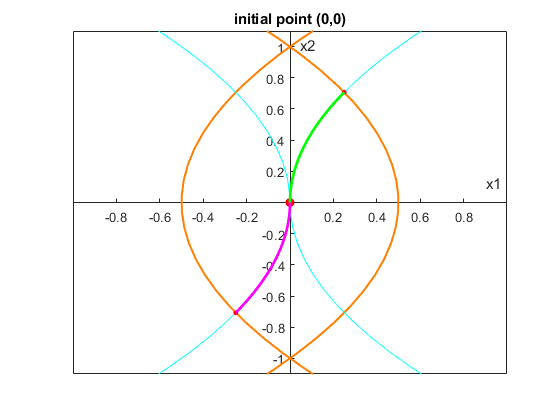
\includegraphics[width=0.5\textwidth]{./figures/6.10.png}
	\caption{Due to symmetry, we see that there are two optimal trajectories from $ (0,0)$ to  $ (0,\pm 1)$.}
\end{figure}
~\begin{figure}[H]
	\centering
	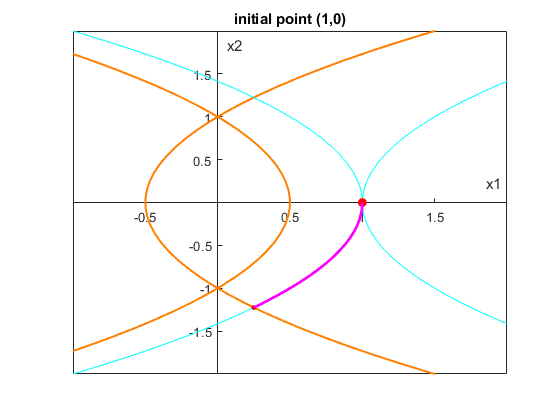
\includegraphics[width=0.49\textwidth]{./figures/6.11.png}
	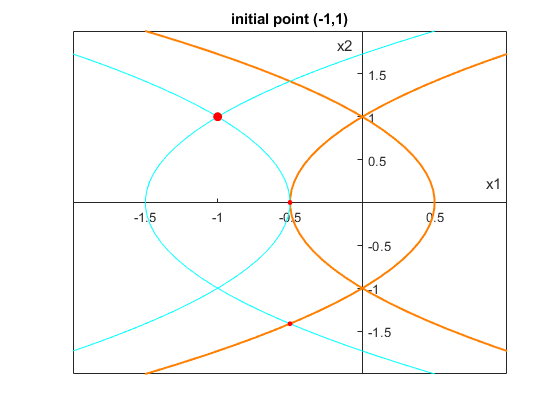
\includegraphics[width=0.49\textwidth]{./figures/6.12.png}
	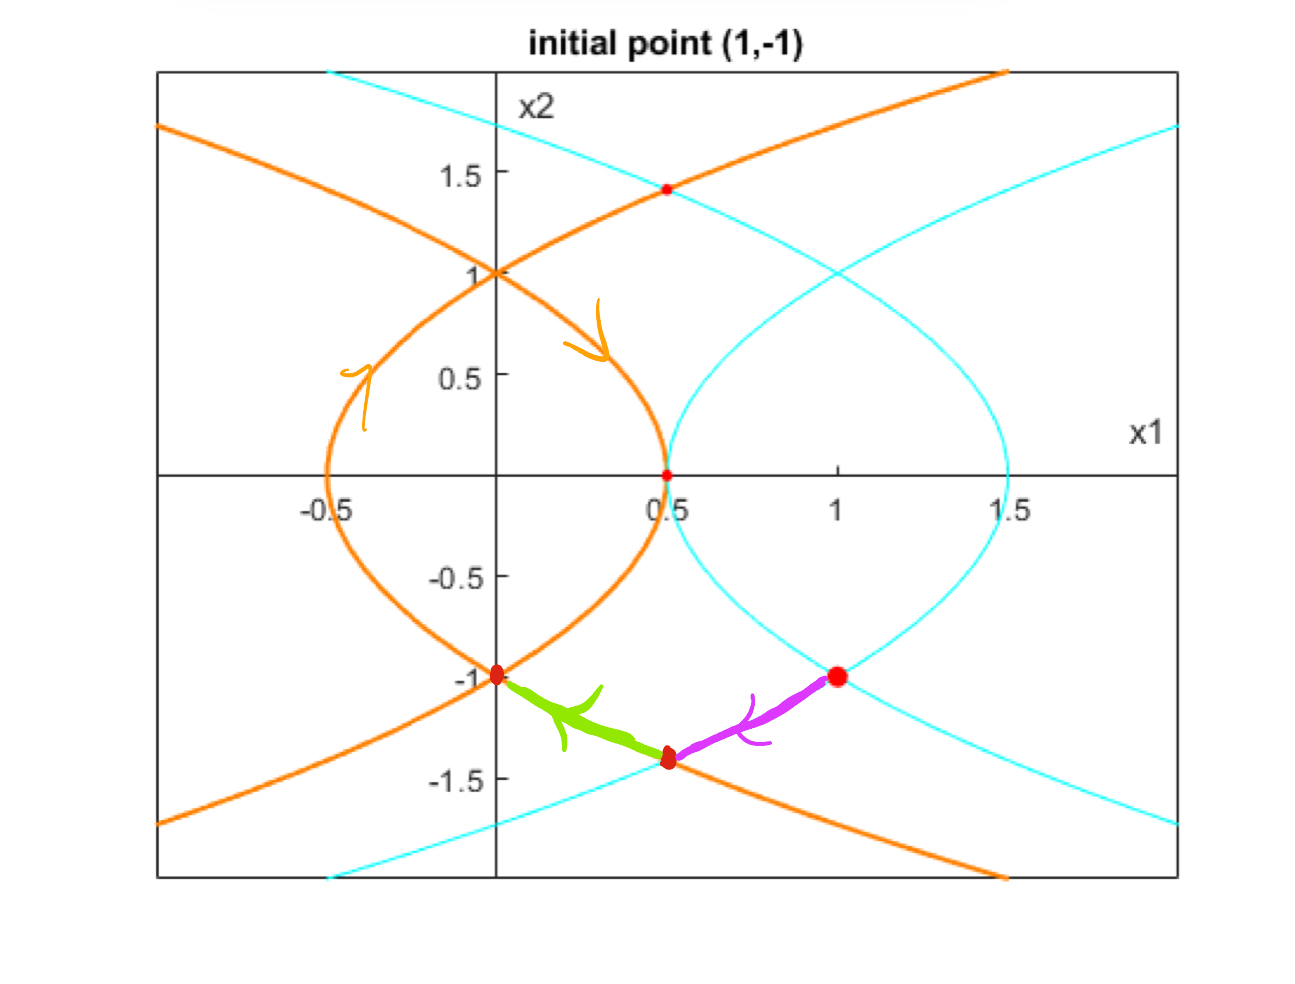
\includegraphics[width=0.49\textwidth]{./figures/6.13.png}
	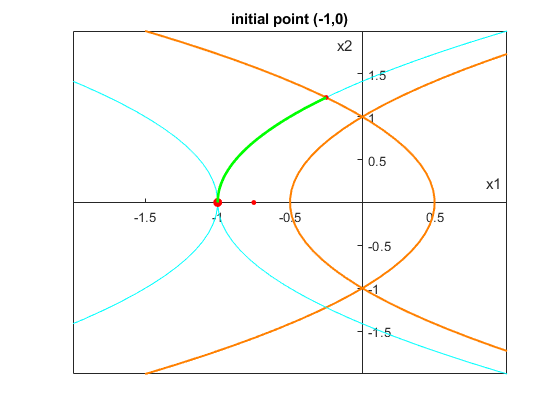
\includegraphics[width=0.49\textwidth]{./figures/6.14.png}
\end{figure}
\end{enumerate}
\end{problem}

\begin{problem}[4]
The Hamiltonian is
\begin{align*}
	H &= t^2 + x^2 + u^2 + pu\\
	H_u &= 2u+p \\
	H_{uu} &= 2 = R_2 >0\\
	H_{ux} &= 0 = R_{12} \\
	H_{x x} &= 2 = R_1 
\end{align*}
Moreover, $ A = \frac{\partial f}{\partial x} =0 $ and $ B = \frac{\partial f}{\partial u} =1$. Recall that for a regular problem, the existence of a conjugate point is equivalent to solution of associated Ricatti equation blowing up. We have
\begin{align*}
	\widetilde{ A} &= A - BR_2^{-1}R_{12}^{T} = 0- \frac{1}{2} \cdot 0 = 0 \\
	\Sigma &= BR_2^{-1}B = \frac{1}{2}\\
	\widetilde{ R} &= R_1- R_{12} R_2^{-1} R_{12}^{T} = 2-0 = 2 
\end{align*}
Thus the Ricatti equation is
\begin{align*}
	-\dot{s} &= \widetilde{ A} ^{T} s + s\widetilde{ A} - s \Sigma s + \widetilde{ R}\\
	-\dot{s} &= -\frac{1}{2} s ^2 + 2
\end{align*}
with $ s(t_f) = 0$. This yields
 \begin{align*}
	s(t) = 2 \tanh(t_f -t), 
\end{align*}
which is bounded! Thus we have no conjugate point.
\end{problem}
\begin{problem}[5]
\begin{enumerate}[label=(\alph*)]
\item The Hamiltonian is
	\begin{align*}
		H = 1+pu
	\end{align*}
with adjoint equation
\begin{align*}
	\dot{p} = 0
\end{align*}
which implies $ p$ is constant. We know  $ p \neq 0$ since otherwise  $ H \equiv 1$ but transversality gives  $ H \equiv 0$, a contradiction. Thus PMP gives
 \begin{align*}
	 u^* &= \begin{cases}
		-1 & p>0\\
		1 & p<0
	\end{cases}\\
	&= - \text{sign}(p)
\end{align*}
\item By letting $ b = - \text{sign}(p) $, we have $ \dot{x} = b$ which yields $ x(t) = bt+x_0$ with $0 =x(t_f) = bt_f + x_0$ so $ x_0 = -bt_f$. So the optimal value $ t_f = -b x_0$.
\item For closed-loop control, we want $ u^* $ in terms of  $ x$. Since we know that $ u$ is a constant, as above from the dynamics we get $ x(t) = ut+x_0$ so boundary condition yields $ u = - \frac{x_0}{ t_f}$. If $ x_0>0$, then since $ t_f >0$, we have $ \dot{x}=u=-1$, so $ x$ decreases as time elapses but remains $ >0$ until $ t_f$. If  $ x_0<0$, $ x$ increases with time but remains $ <0$ until $ t_f$. In either case, we see that $ u^*  = - \text{sign}(x) $. 
\end{enumerate}
\end{problem}

\begin{problem}[6]
The Hamiltonian is
\begin{align*}
	H(x,u,V_x,t) = (xu)^2 + V_x xu .
\end{align*}
The HJB equation is
\begin{align*}
	V_t + \min_u \{(xu)^2 + V_x xu\} =0.
\end{align*}
To find the minimizer, we can set the derivative with respect to $ u$ to zero and obtain
 \begin{align*}
	2x^2 u + V_x x &= 0 \\
	u^* &= - \frac{V_x}{ 2x} ,\quad  x \neq 0
\end{align*}
Then the PDE becomes
\begin{align*}
	4 V_t - V_x^2 =0 . 
\end{align*}
Since $ V(1) = x(1)^2$, we make the guess that the solution has the form $ V(x,t) = p(t) x(t)^2$. Then $ V_t = \dot{p} x^2$ and $ V_x = 2x p(t)$, and we solve the ODE
 \begin{align*}
	4\dot{p}x^2 - p(t)^2 4 x^2 &= 0 \\
	\dot{p} &= p^2 
\end{align*}
with the boundary condition $ p(1) = 1$. The solution is
 \begin{align*}
	p = \frac{1}{2-t} ,
\end{align*}
and the solution to the PDE is
\begin{align*}
	V(x,t) = \frac{x^2}{ 2-t} .
\end{align*}
Thus we have $ V_t = \frac{x^2}{ (2-t)^2}$ and $ V_x = \frac{2x}{ 2-t}$, so the optimal control is 
\begin{align*}
	u^*  = \frac{1}{t-2}.
\end{align*}
Solving the dynamics $ \dot{x} = \frac{x}{t-2}$ with $ x(0)=1$ gives
 \begin{align*}
	x(t) = \frac{2-t}{ 2}
\end{align*}
which indeed doesn't equal 0 in $ [0,1]$. Also $ x(1) = \frac{1}{2}$. The optimal cost is
 \begin{align*}
	J^*  = x(1)^2 + \int_{ 0}^{ 1} \left( \frac{2-t}{ 2} \right)  \frac{1}{t-2} dt = x(1)^2-\frac{1}{2} = \frac{1}{4} - \frac{1}{2} = -\frac{1}{4}.
\end{align*}
\end{problem}

\begin{problem}[7]
The Hamiltonian is
\begin{align*}
	H = \frac{1}{2} x^{T} R_1 x + x^{T} R_{12} u + p ^{T} (Ax+Bu) .
\end{align*}
Recall the following matrix calculus rules $ \frac{d (x^{T}Ax)}{dx} = 2(Ax)^{T} $, or more generally $ \frac{d \langle f(x),g(x) \rangle}{dx} = g(x)^{T} f'(x) + f(x)^{T} g'(x)$. Note this is the derivative/Jacobian, which is the transpose of gradient. The adjoint equation is
\begin{align*}
	\nabla_t p =\dot{p} = -H_x^{T} = -(R_1 x + R_{12} u + A^{T} p)  
\end{align*}
The singular control satisfies
\begin{align*}
	H_u = x^{T}R_{12} + p ^{T}B =0.
\end{align*}
Then
\begin{align*}
	\dot{H_u} = \nabla_t H_u &= \frac{d}{dx} (x^{T} R_{12}) \dot{x} + \frac{d}{dp} (p ^{T}B) \dot{p} \\
	0&= R_{12}^{T}(Ax+Bu) - B^{T}(R_1 x + R_{12} u + A^{T}p) \\
	0&= R_{12}^{T} A x + (R_{12}^{T}B - B^{T}R_{12})u - B^{T}R_1x - B^{T}A^{T}p 
\end{align*}
By GLC, $ u$ can only appear in even degree of differentiation, so for singular control to be optimal we must have  $ R_{12}^{T}B - B^{T} R_{12} = 0$. Then
\begin{align*}
	\ddot{H}_u=\nabla_{tt} H_u &= (R_{12}^{T}A-B^{T}R_1)\dot{x} -B^{T}A^{T}\dot{p} \\ 
	0&= (R_{12}^{T}A-B^{T}R_1)Bu +B^{T}A^{T}R_{12}u + f(x)+g(p) 
\end{align*}
Since $ u$ shows up at degree 2,  $ k=1$. Thus GLC demands
\begin{align*}
	(-1)^{1} \frac{\partial }{\partial u} \ddot{H_u} &\geq 0\\
	(-1) (R_{12}^{T} AB - B^{T}R_1B+B^{T}A^{T}R_{12}) & \geq 0\\
	B^{T}R_1B - R_{12}^{T}AB - B^{T}A^{T}R_{12} &\geq 0
\end{align*}
\end{problem}

\begin{lstlisting}
%%%%%%%%%%%%%%%%%%%%%%%%%%%%%%%%%%%%%%%%%%%%%%%%%%%%%%%%%%%%%%%%%%%%%%%%%%%
%%%%%%%%%%%%%%%%%%%%%%%%%%%%%% Problem 1a %%%%%%%%%%%%%%%%%%%%%%%%%%%%%%%%%
t = zeros(4,2); %store time

%%%%%%%%% initial point at (2,2) %%%%%%%%%
x0 = 2;
y0 = 2;
%time
t1 = 0; %optimal time
t2 = 0; %non-optimal time
%%%%%%%%%%%%%%%%%%%%%%%% optimal trajectory %%%%%%%%%%%%%%%%%%%%%%%%%%%%%%%
%blue circle centered at (-1,0)
th = linspace(0, 2*pi, 100);
R = norm([x0+1,y0]);  %radius
%circle
cx1 = R*cos(th) - 1;
cy1 = R*sin(th);
%find the first intersection of blue circle with switching curve
syms x y
%eyeball the switching curve it intersects with
eqns=[(x-3)^2+y^2==1,(x+1)^2+y^2==R^2];
sol = solve(eqns);
pt1 = [sol.x(1);sol.y(1)]
pt1 = double(pt1);
%first arc of optimal trajectory
th0 = atan(y0/(x0+1)); % initial angle for blue circle
th1 = atan(pt1(2)/(pt1(1)+1)); %first switch angle for blue circle
t1 = t1 + th0-th1; %time is the same as angle
th = linspace( th0, th1, 100);
%trajectory arc 1
trajx1 = R*cos(th) - 1;
trajy1 = R*sin(th);

%green circle centered at (1,0)
th = linspace(0, 2*pi, 100);
R = norm(pt1-[1;0]);  %radius
%circle
cx2 = R*cos(th) + 1;
cy2 = R*sin(th);
%find the next intersection of green circle with switching curve
syms x y
eqns=[(x+1)^2+y^2==1,(x-1)^2+y^2==R^2];
sol = solve(eqns);
pt2 = [sol.x(2);sol.y(2)]
pt2 = double(pt2);
%second arc of optimal trajectory
th0 = atan(pt1(2)/(pt1(1)-1)); % initial angle for green circle
th1 = acos((pt2(1)-1)/R); %first switch angle for green circle
t1 = t1 + th0+2*pi - th1; %time is the same as angle
th = linspace( th0+2*pi, th1, 100);
%trajectory arc 2
trajx2 = R*cos(th) + 1;
trajy2 = R*sin(th);

%semi-circle switching curves
th = linspace( 0, -pi, 100);
R = 1;  %radius
sx1 = R*cos(th) + 3;
sy1 = R*sin(th) ;
sx2 = R*cos(th) + 1;
sy2 = R*sin(th) ;
th = linspace( 0, pi, 100);
sx3 = R*cos(th) - 1;
sy3 = R*sin(th) ;
%third arc of optimal trajectory
th0 = asin(pt2(2)); % initial angle for semicircle
th1 = 0; %terminal angle for for semicircle
t1 = t1+ th0-th1;
th = linspace( th0,th1, 100);
trajx3 = R*cos(th) - 1;
trajy3 = R*sin(th);

figure;
plot(x0,y0,'o',MarkerEdgeColor='r',MarkerFaceColor='r')
hold on
plot(pt1(1),pt1(2),'o',MarkerEdgeColor='r',MarkerFaceColor='r')
plot(pt2(1),pt2(2),'o',MarkerEdgeColor='r',MarkerFaceColor='r')
plot(0,0,'o',MarkerEdgeColor='r',MarkerFaceColor='r')
plot(sx1,sy1,Color=[1 .5 0],LineWidth=1.5); axis equal;
plot(sx2,sy2,Color=[1 .5 0],LineWidth=1.5); 
plot(sx3,sy3,Color=[1 .5 0],LineWidth=1.5); 
plot(cx1,cy1,Color='blue');
plot(trajx1,trajy1,Color='magenta',LineWidth=2);
plot(cx2,cy2,Color='green');
plot(trajx2,trajy2,Color='magenta',LineWidth=2);
plot(trajx3,trajy3,Color='magenta',LineWidth=2);
set(gca, 'XAxisLocation', 'origin')
set(gca, 'YAxisLocation', 'origin')
xlabel('wx1');
ylabel('wx2');
title('optimal trajectory wx1=2');
hold off

%%%%%%%%%%%%%%%%%%%%%%%% non-optimal trajectory %%%%%%%%%%%%%%%%%%%%%%%%%%%
%blue circle centered at (-1,0)
th = linspace(0, 2*pi, 100);
R = norm([x0+1,y0]);  %radius
cx1 = R*cos(th) - 1;
cy1 = R*sin(th);
%find the first intersection of blue circle with switching curve
syms x y
eqns=[y==0,(x+1)^2+y^2==R^2];
sol = solve(eqns);
pt1 = [sol.x(2);sol.y(2)]
pt1 = double(pt1);
%first arc of optimal trajectory
th0 = atan(y0/(x0+1)); % initial angle for blue circle
th1 = atan(pt1(2)/(pt1(1)+1)); %first switch angle for blue circle
t2 = t2 + th0-th1; %time is the same as angle
th = linspace( th0, th1, 100);
trajx1 = R*cos(th) - 1;
trajy1 = R*sin(th);

%green circle centered at (1,0)
th = linspace(0, 2*pi, 100);
R = norm(pt1-[1;0]);  %radius
cx2 = R*cos(th) + 1;
cy2 = R*sin(th);
%find the next intersection of green circle with switching curve
syms x y
eqns=[(x+1)^2+y^2==1,(x-1)^2+y^2==R^2];
sol = solve(eqns);
pt2 = [sol.x(2);sol.y(2)]
pt2 = double(pt2);
%second arc of non-optimal trajectory
th0 = atan(pt1(2)/(pt1(1)-1)); % initial angle for green circle
th1 = acos((pt2(1)-1)/R); %first switch angle for green circle
t2 = t2 + th0+2*pi - th1; %time is the same as angle
th = linspace( th0+2*pi, th1, 100);
trajx2 = R*cos(th) + 1;
trajy2 = R*sin(th);
%Gamma hat switching curves
th = linspace( 0, -pi, 100);
R = 1;  %radius
sx1 = linspace(-5,-2);
sx11 = linspace(2,5);
sy1 = 0*sx1;
sy11 = 0*sx11;
sx2 = R*cos(th) + 1;
sy2 = R*sin(th) ;
th = linspace( 0, pi, 100);
sx3 = R*cos(th) - 1;
sy3 = R*sin(th) ;
%third arc of optimal trajectory
th0 = acos(pt2(1)+1); % initial angle for semicircle
th1 = 0; %terminal angle for for semicircle
t2 = t2+ th0-th1;
th = linspace( th0,th1, 100);
trajx3 = R*cos(th) - 1;
trajy3 = R*sin(th);

figure;
plot(x0,y0,'o',MarkerEdgeColor='r',MarkerFaceColor='r')
hold on
plot(pt1(1),pt1(2),'o',MarkerEdgeColor='r',MarkerFaceColor='r')
plot(pt2(1),pt2(2),'o',MarkerEdgeColor='r',MarkerFaceColor='r')
plot(0,0,'o',MarkerEdgeColor='r',MarkerFaceColor='r')
plot(sx1,sy1,Color=[1 .5 0],LineWidth=1.5); axis equal;
plot(sx11,sy11,Color=[1 .5 0],LineWidth=1.5);
plot(sx2,sy2,Color=[1 .5 0],LineWidth=1.5); 
plot(sx3,sy3,Color=[1 .5 0],LineWidth=1.5); 
plot(cx1,cy1,Color='blue');
plot(trajx1,trajy1,Color='magenta',LineWidth=2);
plot(cx2,cy2,Color='green');
plot(trajx2,trajy2,Color='magenta',LineWidth=2);
plot(trajx3,trajy3,Color='magenta',LineWidth=2);
set(gca, 'XAxisLocation', 'origin')
set(gca, 'YAxisLocation', 'origin')
xlabel('wx1');
ylabel('wx2');
title('non-optimal trajectory wx1=2');
hold off

fprintf('The optimal time is %f, the non-optimal time is %f.\n',t1,t2)

t(1,1) = t1;
t(1,2) = t2;

%%%%%%%%%%%%%%%%%%%%%%%%%%% Problem 1b %%%%%%%%%%%%%%%%%%%%%%%%%%%%%%%%%%%%

%%%%%%% initial point at (3,2) %%%%%%%%%
x0 = 3;
y0 = 2;
%time
t1 = 0; %optimal time
t2 = 0; %non-optimal time
%blue circle centered at (-1,0)
th = linspace(0, 2*pi, 100);
R = norm([x0+1,y0]);  %radius
cx1 = R*cos(th) - 1;
cy1 = R*sin(th);
%find the first intersection of blue circle with switching curve
syms x y
eqns=[(x-3)^2+y^2==1,(x+1)^2+y^2==R^2];
sol = solve(eqns);
pt1 = [sol.x(1);sol.y(1)]
pt1 = double(pt1);
%first arc of optimal trajectory
th0 = atan(y0/(x0+1)); % initial angle for blue circle
th1 = atan(pt1(2)/(pt1(1)+1)); %first switch angle for blue circle
t1 = t1 + th0-th1; %time is the same as angle
th = linspace( th0, th1, 100);
trajx1 = R*cos(th) - 1;
trajy1 = R*sin(th);

%green circle centered at (1,0)
th = linspace(0, 2*pi, 100);
R = norm(pt1-[1;0]);  %radius
cx2 = R*cos(th) + 1;
cy2 = R*sin(th);
%find the next intersection of green circle with switching curve
syms x y
eqns=[(x+1)^2+y^2==1,(x-1)^2+y^2==R^2];
sol = solve(eqns);
pt2 = [sol.x(2);sol.y(2)]
pt2 = double(pt2);
%%%%%%second arc of optimal trajectory
th0 = atan(pt1(2)/(pt1(1)-1)); % initial angle for green circle
th1 = acos((pt2(1)-1)/R); %first switch angle for green circle
t1 = t1 + th0+2*pi - th1; %time is the same as angle
th = linspace( th0+2*pi, th1, 100);
trajx2 = R*cos(th) + 1;
trajy2 = R*sin(th);
%semi-circle switching curves
th = linspace( 0, -pi, 100);
R = 1;  %radius
sx1 = R*cos(th) + 3;
sy1 = R*sin(th) ;
sx2 = R*cos(th) + 1;
sy2 = R*sin(th) ;
th = linspace( 0, pi, 100);
sx3 = R*cos(th) - 1;
sy3 = R*sin(th) ;
%%%%third arc of optimal trajectory
th0 = acos(pt2(1)+1); % initial angle for semicircle
th1 = 0; %terminal angle for for semicircle
t1 = t1+ th0-th1;
th = linspace( th0,th1, 100);
trajx3 = R*cos(th) - 1;
trajy3 = R*sin(th);

figure;
plot(x0,y0,'o',MarkerEdgeColor='r',MarkerFaceColor='r')
hold on
plot(pt1(1),pt1(2),'o',MarkerEdgeColor='r',MarkerFaceColor='r')
plot(pt2(1),pt2(2),'o',MarkerEdgeColor='r',MarkerFaceColor='r')
plot(0,0,'o',MarkerEdgeColor='r',MarkerFaceColor='r')
plot(sx1,sy1,Color=[1 .5 0],LineWidth=1.5); axis equal;
plot(sx2,sy2,Color=[1 .5 0],LineWidth=1.5); 
plot(sx3,sy3,Color=[1 .5 0],LineWidth=1.5); 
plot(cx1,cy1,Color='blue');
plot(trajx1,trajy1,Color='magenta',LineWidth=2);
plot(cx2,cy2,Color='green');
plot(trajx2,trajy2,Color='magenta',LineWidth=2);
plot(trajx3,trajy3,Color='magenta',LineWidth=2);
set(gca, 'XAxisLocation', 'origin')
set(gca, 'YAxisLocation', 'origin')
xlabel('wx1');
ylabel('wx2');
title('optimal trajectory wx1=3');
hold off

%%%%%%%%%%%%%%%%%%%%%%%% non-optimal trajectory %%%%%%%%%%%%%%%%%%%%%%%%%%%
%blue circle centered at (-1,0)
th = linspace(0, 2*pi, 100);
R = norm([x0+1,y0]);  %radius
cx1 = R*cos(th) - 1;
cy1 = R*sin(th);
%find the first intersection of blue circle with switching curve
syms x y
eqns=[y==0,(x+1)^2+y^2==R^2];
sol = solve(eqns);
pt1 = [sol.x(2);sol.y(2)]
pt1 = double(pt1);
%first arc of optimal trajectory
th0 = atan(y0/(x0+1)); % initial angle for blue circle
th1 = atan(pt1(2)/(pt1(1)+1)); %first switch angle for blue circle
t2 = t2 + th0-th1; %time is the same as angle
th = linspace( th0, th1, 100);
trajx1 = R*cos(th) - 1;
trajy1 = R*sin(th);

%green circle centered at (1,0)
th = linspace(0, 2*pi, 100);
R = norm(pt1-[1;0]);  %radius
cx2 = R*cos(th) + 1;
cy2 = R*sin(th);
%find the next intersection of green circle with switching curve
syms x y
eqns=[(x+1)^2+y^2==1,(x-1)^2+y^2==R^2];
sol = solve(eqns);
pt2 = [sol.x(2);sol.y(2)]
pt2 = double(pt2);
%second arc of non-optimal trajectory
th0 = atan(pt1(2)/(pt1(1)-1)); % initial angle for green circle
th1 = acos((pt2(1)-1)/R); %first switch angle for green circle
t2 = t2 + th0+2*pi - th1; %time is the same as angle
th = linspace( th0+2*pi, th1, 100);
trajx2 = R*cos(th) + 1;
trajy2 = R*sin(th);
%Gamma hat switching curves
th = linspace( 0, -pi, 100);
R = 1;  %radius
sx1 = linspace(-6,-2);
sx11 = linspace(2,6);
sy1 = 0*sx1;
sy11 = 0*sx11;
sy1 = 0*sx1;
sx2 = R*cos(th) + 1;
sy2 = R*sin(th) ;
th = linspace( 0, pi, 100);
sx3 = R*cos(th) - 1;
sy3 = R*sin(th) ;
%third arc of optimal trajectory
th0 = acos(pt2(1)+1); % initial angle for semicircle
th1 = 0; %terminal angle for for semicircle
t2 = t2+ th0-th1;
th = linspace( th0,th1, 100);
trajx3 = R*cos(th) - 1;
trajy3 = R*sin(th);

figure;
plot(x0,y0,'o',MarkerEdgeColor='r',MarkerFaceColor='r')
hold on
plot(pt1(1),pt1(2),'o',MarkerEdgeColor='r',MarkerFaceColor='r')
plot(pt2(1),pt2(2),'o',MarkerEdgeColor='r',MarkerFaceColor='r')
plot(0,0,'o',MarkerEdgeColor='r',MarkerFaceColor='r')
plot(sx1,sy1,Color=[1 .5 0],LineWidth=1.5); axis equal;
plot(sx11,sy11,Color=[1 .5 0],LineWidth=1.5);
plot(sx2,sy2,Color=[1 .5 0],LineWidth=1.5); 
plot(sx3,sy3,Color=[1 .5 0],LineWidth=1.5); 
plot(cx1,cy1,Color='blue');
plot(trajx1,trajy1,Color='magenta',LineWidth=2);
plot(cx2,cy2,Color='green');
plot(trajx2,trajy2,Color='magenta',LineWidth=2);
plot(trajx3,trajy3,Color='magenta',LineWidth=2);
set(gca, 'XAxisLocation', 'origin')
set(gca, 'YAxisLocation', 'origin')
xlabel('wx1');
ylabel('wx2');
title('non-optimal trajectory wx1=3');
hold off


t(2,1) = t1;
t(2,2) = t2;

%%%%%%%%%%%%%%%%%%%%%%%% initial point at (4,2) %%%%%%%%%%%%%%%%%%%%%%%%%%%
x0 = 4;
y0 = 2;

%time
t1 = 0; %optimal time
t2 = 0; %non-optimal time
%blue circle centered at (-1,0)
th = linspace(0, 2*pi, 100);
R = norm([x0+1,y0]);  %radius
cx1 = R*cos(th) - 1;
cy1 = R*sin(th);
%find the first intersection of blue circle with switching curve
syms x y
eqns=[(x-5)^2+y^2==1,(x+1)^2+y^2==R^2];
sol = solve(eqns);
pt1 = [sol.x(1);sol.y(1)]
pt1 = double(pt1);
%first arc of optimal trajectory
th0 = atan(y0/(x0+1)); % initial angle for blue circle
th1 = atan(pt1(2)/(pt1(1)+1)); %first switch angle for blue circle
th0-th1
t1 = t1 + th0-th1; %time is the same as angle
th = linspace( th0, th1, 100);
trajx1 = R*cos(th) - 1;
trajy1 = R*sin(th);

%green circle centered at (1,0)
th = linspace(0, 2*pi, 100);
R = norm(pt1-[1;0]);  %radius
cx2 = R*cos(th) + 1;
cy2 = R*sin(th);
%find the next intersection of green circle with switching curve
syms x y
eqns=[(x+3)^2+y^2==1,(x-1)^2+y^2==R^2];
sol = solve(eqns);
pt2 = [sol.x(2);sol.y(2)]
pt2 = double(pt2);
%%%%%%second arc of optimal trajectory
th0 = atan(pt1(2)/(pt1(1)-1)); % initial angle for green circle
th1 = acos((pt2(1)-1)/R); %first switch angle for green circle
th0+2*pi - th1
t1 = t1 + th0+2*pi - th1; %time is the same as angle
th = linspace( th0+2*pi, th1, 100);
trajx2 = R*cos(th) + 1;
trajy2 = R*sin(th);

%blue circle centered at (-1,0)
th = linspace(0, 2*pi, 100);
R = norm(pt2+[1;0]);  %radius
cx3 = R*cos(th) - 1;
cy3 = R*sin(th);
%find the next intersection of blue circle with switching curve
syms x y
eqns=[(x-1)^2+y^2==1,(x+1)^2+y^2==R^2];
sol = solve(eqns);
pt3 = [sol.x(1);sol.y(1)]
pt3 = double(pt3);
%third arc of optimal trajectory
th0 = acos((pt2(1)+1)/R); % initial angle for blue circle
th1 = atan(pt3(2)/(pt3(1)+1)); %first switch angle for blue circle
th0-th1
t1 = t1 + th0-th1; %time is the same as angle
th = linspace( th0, th1, 100);
trajx3 = R*cos(th) - 1;
trajy3 = R*sin(th);

%semi-circle switching curves
th = linspace( 0, -pi, 100);
R = 1;  %radius
sx1 = R*cos(th) + 3;
sy1 = R*sin(th) ;
sx2 = R*cos(th) + 1;
sy2 = R*sin(th) ;
sx3 = R*cos(th) + 5;
sy3 = R*sin(th) ;
th = linspace( 0, pi, 100);
sx4 = R*cos(th) - 1;
sy4 = R*sin(th) ;
sx5 = R*cos(th) - 3;
sy5 = R*sin(th) ;
%%%%fourth arc of optimal trajectory
th0 = -acos(pt3(1)-1); % initial angle for semicircle
th1 = -pi; %terminal angle for for semicircle
abs(th1-th0)
t1 = t1+ abs(th1-th0);
th = linspace( th0,th1, 100);
trajx4 = R*cos(th) + 1;
trajy4 = R*sin(th);

figure;
plot(x0,y0,'o',MarkerEdgeColor='r',MarkerFaceColor='r')
hold on
plot(pt1(1),pt1(2),'o',MarkerEdgeColor='r',MarkerFaceColor='r')
plot(pt2(1),pt2(2),'o',MarkerEdgeColor='r',MarkerFaceColor='r')
plot(pt3(1),pt3(2),'o',MarkerEdgeColor='r',MarkerFaceColor='r')
plot(0,0,'o',MarkerEdgeColor='r',MarkerFaceColor='r')
plot(sx1,sy1,Color=[1 .5 0],LineWidth=1.5); axis equal;
plot(sx2,sy2,Color=[1 .5 0],LineWidth=1.5); 
plot(sx3,sy3,Color=[1 .5 0],LineWidth=1.5); 
plot(sx4,sy4,Color=[1 .5 0],LineWidth=1.5); 
plot(sx5,sy5,Color=[1 .5 0],LineWidth=1.5); 
plot(cx1,cy1,Color='blue');
plot(trajx1,trajy1,Color='magenta',LineWidth=2);
plot(cx2,cy2,Color='green');
plot(trajx2,trajy2,Color='magenta',LineWidth=2);
plot(cx3,cy3,Color='blue');
plot(trajx3,trajy3,Color='magenta',LineWidth=2);
plot(trajx4,trajy4,Color='magenta',LineWidth=2);
set(gca, 'XAxisLocation', 'origin')
set(gca, 'YAxisLocation', 'origin')
xlabel('wx1');
ylabel('wx2');
title('optimal trajectory wx1=4');
hold off

%%%%%%%%%%%%%%%%%%%%%%%% non-optimal trajectory %%%%%%%%%%%%%%%%%%%%%%%%%%%
%blue circle centered at (-1,0)
th = linspace(0, 2*pi, 100);
R = norm([x0+1,y0]);  %radius
cx1 = R*cos(th) - 1;
cy1 = R*sin(th);
%find the first intersection of blue circle with switching curve
syms x y
eqns=[y==0,(x+1)^2+y^2==R^2];
sol = solve(eqns);
pt1 = [sol.x(2);sol.y(2)]
pt1 = double(pt1);
%first arc of optimal trajectory
th0 = atan(y0/(x0+1)); % initial angle for blue circle
th1 = atan(pt1(2)/(pt1(1)+1)); %first switch angle for blue circle
th0-th1
t2 = t2 + th0-th1; %time is the same as angle
th = linspace( th0, th1, 100);
trajx1 = R*cos(th) - 1;
trajy1 = R*sin(th);

%green circle centered at (1,0)
th = linspace(0, 2*pi, 100);
R = norm(pt1-[1;0]);  %radius
cx2 = R*cos(th) + 1;
cy2 = R*sin(th);
%find the next intersection of green circle with switching curve
syms x y
eqns=[y==0,(x-1)^2+y^2==R^2];
sol = solve(eqns);
pt2 = [sol.x(1);sol.y(1)]
pt2 = double(pt2);
%second arc of non-optimal trajectory
th0 = atan(pt1(2)/(pt1(1)-1)); % initial angle for green circle
th1 = acos((pt2(1)-1)/R); %first switch angle for green circle
th0+2*pi - th1
t2 = t2 + th0+2*pi - th1; %time is the same as angle
th = linspace( th0+2*pi, th1, 100);
trajx2 = R*cos(th) + 1;
trajy2 = R*sin(th);

%blue circle centered at (-1,0)
th = linspace(0, 2*pi, 100);
R = norm(pt2+[1;0]);  %radius
cx3 = R*cos(th) - 1;
cy3 = R*sin(th);
%find the next intersection of blue circle with switching curve
syms x y
eqns=[(x-1)^2+y^2==1,(x+1)^2+y^2==R^2];
sol = solve(eqns);
pt3 = [sol.x(1);sol.y(1)]
pt3 = double(pt3);
%third arc of non-optimal trajectory
th0 = acos((pt2(1)+1)/R); % initial angle for blue circle
th1 = atan(pt3(2)/(pt3(1)+1)); %first switch angle for blue circle
th0-th1
t2 = t2 + th0-th1; %time is the same as angle
th = linspace( th0, th1, 100);
trajx3 = R*cos(th) - 1;
trajy3 = R*sin(th);

%Gamma hat switching curves
th = linspace( 0, -pi, 100);
R = 1;  %radius
sx1 = linspace(-7,-2);
sx11 = linspace(2,7);
sy1 = 0*sx1;
sy11 = 0*sx11;
sy1 = 0*sx1;
sx2 = R*cos(th) + 1;
sy2 = R*sin(th) ;
th = linspace( 0, pi, 100);
sx3 = R*cos(th) - 1;
sy3 = R*sin(th) ;

%%%%fourth arc of non-optimal trajectory
th0 = -acos(pt3(1)-1); % initial angle for semicircle
th1 = -pi; %terminal angle for for semicircle
abs(th1-th0)
t2 = t2 + abs(th1-th0);
th = linspace( th0,th1, 100);
trajx4 = R*cos(th) + 1;
trajy4 = R*sin(th);

figure;
plot(x0,y0,'o',MarkerEdgeColor='r',MarkerFaceColor='r')
hold on
plot(pt1(1),pt1(2),'o',MarkerEdgeColor='r',MarkerFaceColor='r')
plot(pt2(1),pt2(2),'o',MarkerEdgeColor='r',MarkerFaceColor='r')
plot(pt3(1),pt3(2),'o',MarkerEdgeColor='r',MarkerFaceColor='r')
plot(0,0,'o',MarkerEdgeColor='r',MarkerFaceColor='r')
plot(sx1,sy1,Color=[1 .5 0],LineWidth=1.5); axis equal;
plot(sx11,sy11,Color=[1 .5 0],LineWidth=1.5);
plot(sx2,sy2,Color=[1 .5 0],LineWidth=1.5); 
plot(sx3,sy3,Color=[1 .5 0],LineWidth=1.5); 
plot(cx1,cy1,Color='blue');
plot(trajx1,trajy1,Color='magenta',LineWidth=2);
plot(cx2,cy2,Color='green');
plot(cx3,cy3,Color='blue');
plot(trajx2,trajy2,Color='magenta',LineWidth=2);
plot(trajx3,trajy3,Color='magenta',LineWidth=2);
plot(trajx4,trajy4,Color='magenta',LineWidth=2);
set(gca, 'XAxisLocation', 'origin')
set(gca, 'YAxisLocation', 'origin')
xlabel('wx1');
ylabel('wx2');
title('non-optimal trajectory wx1=4');
hold off

t(3,1) = t1;
t(3,2) = t2;
%%%%%%%%%%%%%%%%%%%%%% initial point at (5,2) %%%%%%%%%%%%%%%%%%%%%%%%%%%%%
x0 = 5;
y0 = 2;

%time
t1 = 0; %optimal time
t2 = 0; %non-optimal time
%blue circle centered at (-1,0)
th = linspace(0, 2*pi, 100);
R = norm([x0+1,y0]);  %radius
cx1 = R*cos(th) - 1;
cy1 = R*sin(th);
%find the first intersection of blue circle with switching curve
syms x y
eqns=[(x-5)^2+y^2==1,(x+1)^2+y^2==R^2];
sol = solve(eqns);
pt1 = [sol.x(1);sol.y(1)]
pt1 = double(pt1);
%first arc of optimal trajectory
th0 = atan(y0/(x0+1)); % initial angle for blue circle
th1 = atan(pt1(2)/(pt1(1)+1)); %first switch angle for blue circle
t1 = t1 + th0-th1; %time is the same as angle
th = linspace( th0, th1, 100);
trajx1 = R*cos(th) - 1;
trajy1 = R*sin(th);

%green circle centered at (1,0)
th = linspace(0, 2*pi, 100);
R = norm(pt1-[1;0]);  %radius
cx2 = R*cos(th) + 1;
cy2 = R*sin(th);
%find the next intersection of green circle with switching curve
syms x y
eqns=[(x+3)^2+y^2==1,(x-1)^2+y^2==R^2];
sol = solve(eqns);
pt2 = [sol.x(2);sol.y(2)]
pt2 = double(pt2);
%%%%%%second arc of optimal trajectory
th0 = atan(pt1(2)/(pt1(1)-1)); % initial angle for green circle
th1 = acos((pt2(1)-1)/R); %first switch angle for green circle
t1 = t1 + th0+2*pi - th1; %time is the same as angle
th = linspace( th0+2*pi, th1, 100);
trajx2 = R*cos(th) + 1;
trajy2 = R*sin(th);

%blue circle centered at (-1,0)
th = linspace(0, 2*pi, 100);
R = norm(pt2+[1;0]);  %radius
cx3 = R*cos(th) - 1;
cy3 = R*sin(th);
%find the next intersection of blue circle with switching curve
syms x y
eqns=[(x-1)^2+y^2==1,(x+1)^2+y^2==R^2];
sol = solve(eqns);
pt3 = [sol.x(1);sol.y(1)]
pt3 = double(pt3);
%third arc of optimal trajectory
th0 = acos((pt2(1)+1)/R); % initial angle for blue circle
th1 = atan(pt3(2)/(pt3(1)+1)); %first switch angle for blue circle
t1 = t1 + th0-th1; %time is the same as angle
th = linspace( th0, th1, 100);
trajx3 = R*cos(th) - 1;
trajy3 = R*sin(th);

%semi-circle switching curves
th = linspace( 0, -pi, 100);
R = 1;  %radius
sx1 = R*cos(th) + 3;
sy1 = R*sin(th) ;
sx2 = R*cos(th) + 1;
sy2 = R*sin(th) ;
sx3 = R*cos(th) + 5;
sy3 = R*sin(th) ;
th = linspace( 0, pi, 100);
sx4 = R*cos(th) - 1;
sy4 = R*sin(th) ;
sx5 = R*cos(th) - 3;
sy5 = R*sin(th) ;
%%%%fourth arc of optimal trajectory
th0 = -acos(pt3(1)-1); % initial angle for semicircle
th1 = -pi; %terminal angle for for semicircle
t1 = t1+ abs(th1-th0);
th = linspace( th0,th1, 100);
trajx4 = R*cos(th) + 1;
trajy4 = R*sin(th);

figure;
plot(x0,y0,'o',MarkerEdgeColor='r',MarkerFaceColor='r')
hold on
plot(pt1(1),pt1(2),'o',MarkerEdgeColor='r',MarkerFaceColor='r')
plot(pt2(1),pt2(2),'o',MarkerEdgeColor='r',MarkerFaceColor='r')
plot(pt3(1),pt3(2),'o',MarkerEdgeColor='r',MarkerFaceColor='r')
plot(0,0,'o',MarkerEdgeColor='r',MarkerFaceColor='r')
plot(sx1,sy1,Color=[1 .5 0],LineWidth=1.5); axis equal;
plot(sx2,sy2,Color=[1 .5 0],LineWidth=1.5); 
plot(sx3,sy3,Color=[1 .5 0],LineWidth=1.5); 
plot(sx4,sy4,Color=[1 .5 0],LineWidth=1.5); 
plot(sx5,sy5,Color=[1 .5 0],LineWidth=1.5); 
plot(cx1,cy1,Color='blue');
plot(trajx1,trajy1,Color='magenta',LineWidth=2);
plot(cx2,cy2,Color='green');
plot(trajx2,trajy2,Color='magenta',LineWidth=2);
plot(cx3,cy3,Color='blue');
plot(trajx3,trajy3,Color='magenta',LineWidth=2);
plot(trajx4,trajy4,Color='magenta',LineWidth=2);
set(gca, 'XAxisLocation', 'origin')
set(gca, 'YAxisLocation', 'origin')
xlabel('wx1');
ylabel('wx2');
title('optimal trajectory wx1=5');
hold off

%%%%%%%%%%%%%%%%%%%%%%%% non-optimal trajectory %%%%%%%%%%%%%%%%%%%%%%%%%%%
%blue circle centered at (-1,0)
th = linspace(0, 2*pi, 100);
R = norm([x0+1,y0]);  %radius
cx1 = R*cos(th) - 1;
cy1 = R*sin(th);
%find the first intersection of blue circle with switching curve
syms x y
eqns=[y==0,(x+1)^2+y^2==R^2];
sol = solve(eqns);
pt1 = [sol.x(2);sol.y(2)]
pt1 = double(pt1);
%first arc of non-optimal trajectory
th0 = atan(y0/(x0+1)); % initial angle for blue circle
th1 = atan(pt1(2)/(pt1(1)+1)); %first switch angle for blue circle
t2 = t2 + th0-th1; %time is the same as angle
th = linspace( th0, th1, 100);
trajx1 = R*cos(th) - 1;
trajy1 = R*sin(th);

%green circle centered at (1,0)
th = linspace(0, 2*pi, 100);
R = norm(pt1-[1;0]);  %radius
cx2 = R*cos(th) + 1;
cy2 = R*sin(th);
%find the next intersection of green circle with switching curve
syms x y
eqns=[y==0,(x-1)^2+y^2==R^2];
sol = solve(eqns);
pt2 = [sol.x(1);sol.y(1)]
pt2 = double(pt2);
%second arc of non-optimal trajectory
th0 = atan(pt1(2)/(pt1(1)-1)); % initial angle for green circle
th1 = acos((pt2(1)-1)/R); %first switch angle for green circle
t2 = t2 + th0+2*pi - th1; %time is the same as angle
th = linspace( th0+2*pi, th1, 100);
trajx2 = R*cos(th) + 1;
trajy2 = R*sin(th);

%blue circle centered at (-1,0)
th = linspace(0, 2*pi, 100);
R = norm(pt2+[1;0]);  %radius
cx3 = R*cos(th) - 1;
cy3 = R*sin(th);
%find the next intersection of blue circle with switching curve
syms x y
eqns=[(x-1)^2+y^2==1,(x+1)^2+y^2==R^2];
sol = solve(eqns);
pt3 = [sol.x(1);sol.y(1)]
pt3 = double(pt3);
%third arc of non-optimal trajectory
th0 = acos((pt2(1)+1)/R); % initial angle for blue circle
th1 = atan(pt3(2)/(pt3(1)+1)); %first switch angle for blue circle
t2 = t2 + th0-th1; %time is the same as angle
th = linspace( th0, th1, 100);
trajx3 = R*cos(th) - 1;
trajy3 = R*sin(th);

%Gamma hat switching curves
th = linspace( 0, -pi, 100);
R = 1;  %radius
sx1 = linspace(-8,-2);
sx11 = linspace(2,8);
sy1 = 0*sx1;
sy11 = 0*sx11;
sy1 = 0*sx1;
sx2 = R*cos(th) + 1;
sy2 = R*sin(th) ;
th = linspace( 0, pi, 100);
sx3 = R*cos(th) - 1;
sy3 = R*sin(th) ;

%%%%fourth arc of non-optimal trajectory
th0 = -acos(pt3(1)-1); % initial angle for semicircle
th1 = -pi; %terminal angle for for semicircle
t2 = t2+ abs(th1-th0);
th = linspace( th0,th1, 100);
trajx4 = R*cos(th) + 1;
trajy4 = R*sin(th);

figure;
plot(x0,y0,'o',MarkerEdgeColor='r',MarkerFaceColor='r')
hold on
plot(pt1(1),pt1(2),'o',MarkerEdgeColor='r',MarkerFaceColor='r')
plot(pt2(1),pt2(2),'o',MarkerEdgeColor='r',MarkerFaceColor='r')
plot(pt3(1),pt3(2),'o',MarkerEdgeColor='r',MarkerFaceColor='r')
plot(0,0,'o',MarkerEdgeColor='r',MarkerFaceColor='r')
plot(sx1,sy1,Color=[1 .5 0],LineWidth=1.5); axis equal;
plot(sx11,sy11,Color=[1 .5 0],LineWidth=1.5);
plot(sx2,sy2,Color=[1 .5 0],LineWidth=1.5); 
plot(sx3,sy3,Color=[1 .5 0],LineWidth=1.5); 
plot(cx1,cy1,Color='blue');
plot(trajx1,trajy1,Color='magenta',LineWidth=2);
plot(cx2,cy2,Color='green');
plot(cx3,cy3,Color='blue');
plot(trajx2,trajy2,Color='magenta',LineWidth=2);
plot(trajx3,trajy3,Color='magenta',LineWidth=2);
plot(trajx4,trajy4,Color='magenta',LineWidth=2);
set(gca, 'XAxisLocation', 'origin')
set(gca, 'YAxisLocation', 'origin')
xlabel('wx1');
ylabel('wx2');
title('non-optimal trajectory wx1=5');
hold off

t(4,1) = t1;
t(4,2) = t2;

figure;
plot(t(:,2)./t(:,1)*100)
ylabel('percentage');
xlabel('wx1-1');
title('time ratio as wx1 increases');
%%%%%%%%%%%%%%%%%%%%%%%%%%%%%%%%%%%%%%%%%%%%%%%%%%%%%%%%%%%%%%%%%%%%%%%%%%%
%%%%%%%%%%%%%%%%%%%%%%%%% Problem 2 %%%%%%%%%%%%%%%%%%%%%%%%%%%%%%%%%%%%%%%
%a
syms x y
eqns = [x==-1/2*(y+1/2)^2-1/2*(y+1/2),x==-2*y];
sol2 = solve(eqns);
sol2.x
sol2.y
eqns = [x==1/2*(y+1/2)^2-3/2*(y+1/2),x==-2*y];
sol2 = solve(eqns);
sol2.x
sol2.y
%b
eqns = [x==1/2*(y+1/2)^2-3/2*(y+1/2),x==-1/2*y^2-y];
sol2 = solve(eqns);
sol2.x
sol2.y
pt = [sol2.x(2);sol2.y(2)];
pt = double(pt)
%%%%%%%%%%%%%%%%%%%%%%%%%%%%%%%%%%%%%%%%%%%%%%%%%%%%%%%%%%%%%%%%%%%%%%%%%%%
%%%%%%%%%%%%%%%%%%%%%%%%% Problem 3 %%%%%%%%%%%%%%%%%%%%%%%%%%%%%%%%%%%%%%%
t = linspace(-2,2);
x0 = 0;
y0 = 1;
%up
Gamma1xf =@(t) 0.5*t.^2 + y0*t + x0;
Gamma1yf =@(t) t + y0;
%down
Gamma2xf =@(t) -0.5*t.^2 + y0*t + x0;
Gamma2yf =@(t) -t + y0;
Gamma1x = Gamma1xf(t);
Gamma1y = Gamma1yf(t);
Gamma2x = Gamma2xf(t);
Gamma2y = Gamma2yf(t);

figure;
hold on
plot(Gamma2x,Gamma2y,Color=[1 .5 0],LineWidth=1.5)
for n=1:5
    k=2*n/3;
    plot(Gamma1x-k,Gamma1y,Color='cyan')
    plot(Gamma1x+k,Gamma1y,Color='cyan')
    plot(Gamma2x-k,Gamma2y,Color='cyan')
    plot(Gamma2x+k,Gamma2y,Color='cyan')
end
set(gca, 'XAxisLocation', 'origin')
set(gca, 'YAxisLocation', 'origin')
xlabel('x1');
ylabel('x2');
title('switching curves');
axis([-4,4,-3,3]);

t = linspace(-2,2);
x0 = 0;
y0 = -1;
%up
Gamma1xf =@(t) 0.5*t.^2 + y0*t + x0;
Gamma1yf =@(t) t + y0;
%down
Gamma2xf =@(t) -0.5*t.^2 + y0*t + x0;
Gamma2yf =@(t) -t + y0;
Gamma1x = Gamma1xf(t);
Gamma1y = Gamma1yf(t);
Gamma2x = Gamma2xf(t);
Gamma2y = Gamma2yf(t);

plot(Gamma1x,Gamma1y,Color=[1 .5 0],LineWidth=1.5)
for n=1:5
    k=2*n/3;
    plot(Gamma1x-k,Gamma1y,Color='cyan')
    plot(Gamma1x+k,Gamma1y,Color='cyan')
    plot(Gamma2x-k,Gamma2y,Color='cyan')
    plot(Gamma2x+k,Gamma2y,Color='cyan')
end
hold off

%%%%%%%%%%% initial (0,0) %%%%%%%%%%%%
x0 = 0;
y0 = 0;
upx =@(t) 0.5*t.^2 + y0*t + x0;
upy =@(t) t + y0;
downx =@(t) -0.5*t.^2 + y0*t + x0;
downy =@(t) -t + y0;

%u=-1 goes down, intersects Gamma2 u=1 goes up
eqns = [x-(x0+1/2*y0^2)==-1/2*(y)^2,x+1/2==1/2*(y)^2];
sol31 = solve(eqns);
sol31.x
sol31.y
pt1 = [sol31.x(1);sol31.y(1)]; %pick the lowest x2 to go up
pt1 = double(pt1);
tf1 = -pt1(2);
t1 = linspace(0,tf1);

%u=1 goes up, intersects Gamma1 u=-1 goes down
eqns = [x-(x0-1/2*y0^2)==1/2*(y)^2,x-1/2==-1/2*(y)^2];
sol32 = solve(eqns);
sol32.x
sol32.y
pt2 = [sol32.x(1);sol32.y(2)]; %pick the highest x2 to go down
pt2 = double(pt2);
tf2 = pt2(2);
t2 = linspace(0,tf2);
figure;
plot(Gamma1x,Gamma1y,Color=[1 .5 0],LineWidth=1.5)
hold on
plot(Gamma2x,Gamma2y,Color=[1 .5 0],LineWidth=1.5)
plot(upx(t),upy(t),Color='cyan')
plot(downx(t),downy(t),Color='cyan')
plot(x0,y0,'o',MarkerEdgeColor='r',MarkerFaceColor='r',MarkerSize=6)
plot(pt1(1),pt1(2),'o',MarkerEdgeColor='r',MarkerFaceColor='r',MarkerSize=3)
plot(pt2(1),pt2(2),'o',MarkerEdgeColor='r',MarkerFaceColor='r',MarkerSize=3)
plot(downx(t1),downy(t1),Color='magenta',LineWidth=2)
plot(upx(t2),upy(t2),Color='green',LineWidth=2)
set(gca, 'XAxisLocation', 'origin')
set(gca, 'YAxisLocation', 'origin')
xlabel('x1');
ylabel('x2');
title('initial point (0,0)');
axis([-1,1,-1.1,1.1]);
hold off


%%%%%%%%%%% initial (1,0) %%%%%%%%%%%%
x0 = 1;
y0 = 0;
upx =@(t) 0.5*t.^2 + y0*t + x0;
upy =@(t) t + y0;
downx =@(t) -0.5*t.^2 + y0*t + x0;
downy =@(t) -t + y0;

%u=-1 goes down, intersects Gamma2 u=1 goes up
eqns = [x-(x0+1/2*y0^2)==-1/2*(y)^2,x+1/2==1/2*(y)^2];
sol31 = solve(eqns);
sol31.x
sol31.y
pt1 = [sol31.x(1);sol31.y(1)]; %pick the lowest x2 to go up
pt1 = double(pt1);
tf1 = -pt1(2);
t1 = linspace(0,tf1);

%u=1 goes up, intersects Gamma1 u=-1 goes down
eqns = [x-(x0-1/2*y0^2)==1/2*(y)^2,x-1/2==-1/2*(y)^2];
%no solution!
figure;
plot(Gamma1x,Gamma1y,Color=[1 .5 0],LineWidth=1.5)
hold on
plot(Gamma2x,Gamma2y,Color=[1 .5 0],LineWidth=1.5)
plot(upx(t),upy(t),Color='cyan')
plot(downx(t),downy(t),Color='cyan')
plot(x0,y0,'o',MarkerEdgeColor='r',MarkerFaceColor='r',MarkerSize=6)
plot(pt1(1),pt1(2),'o',MarkerEdgeColor='r',MarkerFaceColor='r',MarkerSize=3)
plot(downx(t1),downy(t1),Color='magenta',LineWidth=2)
set(gca, 'XAxisLocation', 'origin')
set(gca, 'YAxisLocation', 'origin')
xlabel('x1');
ylabel('x2');
title('initial point (1,0)');
axis([-1,2,-2,2]);
hold off

%%%%%%%%%%% initial (-1,1) %%%%%%%%%%%%
x0 = -1;
y0 = 1;
upx =@(t) 0.5*t.^2 + y0*t + x0;
upy =@(t) t + y0;
downx =@(t) -0.5*t.^2 + y0*t + x0;
downy =@(t) -t + y0;

%u=-1 goes down, intersects Gamma2 u=1 goes up
eqns = [x-(x0+1/2*y0^2)==-1/2*(y)^2,x+1/2==1/2*(y)^2];
sol31 = solve(eqns);
sol31.x
sol31.y
pt1 = [sol31.x(1);sol31.y(1)]; %pick the lowest x2 to go up
pt1 = double(pt1);
tf1 = -pt1(2);
t1 = linspace(0,tf1);

%u=1 goes up, intersects Gamma1 u=-1 goes down
eqns = [x-(x0-1/2*y0^2)==1/2*(y)^2,x-1/2==-1/2*(y)^2];
sol32 = solve(eqns);
sol32.x
sol32.y
pt2 = [sol32.x(1);sol32.y(2)]; %pick the highest x2 to go down
pt2 = double(pt2);
tf2 = pt2(2);
t2 = linspace(0,tf2);
figure;
plot(Gamma1x,Gamma1y,Color=[1 .5 0],LineWidth=1.5)
hold on
plot(Gamma2x,Gamma2y,Color=[1 .5 0],LineWidth=1.5)
plot(upx(t),upy(t),Color='cyan')
plot(downx(t),downy(t),Color='cyan')
plot(x0,y0,'o',MarkerEdgeColor='r',MarkerFaceColor='r',MarkerSize=6)
plot(pt1(1),pt1(2),'o',MarkerEdgeColor='r',MarkerFaceColor='r',MarkerSize=3)
plot(pt2(1),pt2(2),'o',MarkerEdgeColor='r',MarkerFaceColor='r',MarkerSize=3)
plot(downx(t1),downy(t1),Color='magenta',LineWidth=2)
set(gca, 'XAxisLocation', 'origin')
set(gca, 'YAxisLocation', 'origin')
xlabel('x1');
ylabel('x2');
title('initial point (-1,1)');
axis([-2,1,-2,2]);
hold off

%%%%%%%%%%% initial (1,-1) %%%%%%%%%%%%
x0 = 1;
y0 = -1;

upx =@(t) 0.5*t.^2 + y0*t + x0;
upy =@(t) t + y0;
downx =@(t) -0.5*t.^2 + y0*t + x0;
downy =@(t) -t + y0;

%u=-1 goes down, intersects Gamma2 u=1 goes up
eqns = [x-(x0+1/2*y0^2)==-1/2*(y)^2,x+1/2==1/2*(y)^2];
sol31 = solve(eqns);
sol31.x
sol31.y
pt1 = [sol31.x(1);sol31.y(1)]; %pick the lowest x2 to go up
pt1 = double(pt1);
tf1 = -pt1(2);
t1 = linspace(0,tf1);

%u=1 goes up, intersects Gamma1 u=-1 goes down
eqns = [x-(x0-1/2*y0^2)==1/2*(y)^2,x-1/2==-1/2*(y)^2];
sol32 = solve(eqns);
sol32.x
sol32.y
pt2 = [sol32.x(1);sol32.y(1)]; %pick the highest x2 to go down
pt2 = double(pt2);
tf2 = pt2(2);
t2 = linspace(0,tf2);
figure;
plot(Gamma1x,Gamma1y,Color=[1 .5 0],LineWidth=1.5)
hold on
plot(Gamma2x,Gamma2y,Color=[1 .5 0],LineWidth=1.5)
plot(upx(t),upy(t),Color='cyan')
plot(downx(t),downy(t),Color='cyan')
plot(x0,y0,'o',MarkerEdgeColor='r',MarkerFaceColor='r',MarkerSize=6)
plot(pt1(1),pt1(2),'o',MarkerEdgeColor='r',MarkerFaceColor='r',MarkerSize=3)
plot(pt2(1),pt2(2),'o',MarkerEdgeColor='r',MarkerFaceColor='r',MarkerSize=3)
set(gca, 'XAxisLocation', 'origin')
set(gca, 'YAxisLocation', 'origin')
xlabel('x1');
ylabel('x2');
title('initial point (1,-1)');
axis([-1,2,-2,2]);
hold off

%%%%%%%%%%% initial (-1,0) %%%%%%%%%%%%
x0 = -1;
y0 = 0;
upx =@(t) 0.5*t.^2 + y0*t + x0;
upy =@(t) t + y0;
downx =@(t) -0.5*t.^2 + y0*t + x0;
downy =@(t) -t + y0;

%u=-1 goes down, intersects Gamma2 u=1 goes up
eqns = [x-(x0+1/2*y0^2)==-1/2*(y)^2,x+1/2==1/2*(y)^2];
sol31 = solve(eqns);
sol31.x
sol31.y
pt1 = [sol31.x(1);sol31.y(1)]; %pick the lowest x2 to go up
pt1 = double(pt1);
tf1 = -pt1(2);
t1 = linspace(0,tf1);

%u=1 goes up, intersects Gamma1 u=-1 goes down
eqns = [x-(x0-1/2*y0^2)==1/2*(y)^2,x-1/2==-1/2*(y)^2];
sol32 = solve(eqns);
sol32.x
sol32.y
pt2 = [sol32.x(1);sol32.y(2)]; %pick the highest x2 to go down
pt2 = double(pt2);
tf2 = pt2(2);
t2 = linspace(0,tf2);
figure;
plot(Gamma1x,Gamma1y,Color=[1 .5 0],LineWidth=1.5)
hold on
plot(Gamma2x,Gamma2y,Color=[1 .5 0],LineWidth=1.5)
plot(upx(t),upy(t),Color='cyan')
plot(downx(t),downy(t),Color='cyan')
plot(x0,y0,'o',MarkerEdgeColor='r',MarkerFaceColor='r',MarkerSize=6)
plot(pt1(1),pt1(2),'o',MarkerEdgeColor='r',MarkerFaceColor='r',MarkerSize=3)
plot(pt2(1),pt2(2),'o',MarkerEdgeColor='r',MarkerFaceColor='r',MarkerSize=3)
plot(upx(t2),upy(t2),Color='green',LineWidth=2)
set(gca, 'XAxisLocation', 'origin')
set(gca, 'YAxisLocation', 'origin')
xlabel('x1');
ylabel('x2');
title('initial point (-1,0)');
axis([-2,1,-2,2]);
hold off
\end{lstlisting}
\end{document}
